
\documentclass[12pt,a4paper]{article} 

\usepackage{float,times,graphicx,mathtools}
\usepackage{amsmath}
\usepackage{amsfonts}
\usepackage{amssymb}
\usepackage{latexsym}
\usepackage{epsfig}
\usepackage{graphicx}
\usepackage{caption}
\usepackage{subcaption}
\usepackage{color}
\usepackage{pdfpages}
\usepackage{natbib}
\usepackage[space]{grffile}
\usepackage{wrapfig}
\usepackage{subcaption}
\usepackage{url}
\usepackage{bbm}
\usepackage{tikzsymbols}

\DeclareMathOperator{\logit}{logit}
\DeclareMathOperator{\tr}{tr}
\bibpunct[, ]{(}{)}{;}{a}{,}{,}
\graphicspath{{../}}  
\addtolength{\oddsidemargin}{-1in}
	\addtolength{\evensidemargin}{-1in}
	\addtolength{\textwidth}{1.75in}
	\addtolength{\topmargin}{-1.3in}
	\addtolength{\textheight}{2in}
\date{\vspace{-5ex}}
\begin{document}

\begin{itemize}
\item Stan is still giving divergent transitions warnings whenever DEF is included, will come back to that later
\item Tried fixing the same LQ $k$ for all periods, while allowing DEF to vary over time as suggested, and fitted to BF female DHS data
\begin{align*}
 k &\sim N(0,1) \\ ~ \\
\log(h) &= IGME_h + \sigma_h AR1(\rho_h),\\
\sigma_h &\sim IG(1,0.0109), \\
\rho_h &\sim N(0,10), \\ ~ \\
\log(i) &= \mu_i + \sigma_i AR1(\rho_i),\\
\sigma_i &\sim IG(1, 5), \\
\text{logit}(\rho_i) &\sim N(0, 10), \qquad i \in \{D, E, F \} 
\end{align*}
\begin{itemize}
\item[--] rather sensitive to initial values, wasted much time trying to see what works \Changey{-1.5}
	\begin{itemize}
\item[1)] $\mu_i$ estimated as fixed effects without prior $\rightarrow \mu_D \approx \log(0.0006), \, \mu_E \approx \log(4), \, \mu_F \approx \log(641)$, obviously insensible results \\

\item[2)] tried $\mu_i$ treated as constants and fixed at ${\mu_D = \log(\textcolor{blue}{0.005}), \, \mu_E = \log(8), \, \mu_F = \log(35)}$ \begin{itemize}
 \item[\rightarrow] still gives high values of $F (\approx 120)$, often wouldn't converge unless $E$ fixed at higher values \\ \end{itemize}

\item[3)] tried $\mu_i$ treated as constants and fixed at ${\mu_D = \log(\textcolor{red}{0.0005}), \, \mu_E = \log(8), \, \mu_F = \log(35)}$ \begin{itemize} \item[\rightarrow] gives more sensible $F (\approx 16 \text{ to } 33)$ but wider spread $E$ \\ \end{itemize} 

\item[4)] given vague normal priors on $\mu_i \sim N(\eta_i, 30)$ with $\eta_D = \log(0.0005), \, \eta_E = \log(8), \, \eta_F = \log(35)$ \begin{itemize}
\item[\rightarrow] $\mu_i$ estimated as random effects, $F \approx 164$
\item[\rightarrow] $\mu_i$ estimated as fixed effects, $F \approx 204$ \\
 \end{itemize}

\item[5)] given tight normal priors on $\mu_F \sim N(log(35), 0.25)$ (tighter than that wouldn't converge) \begin{itemize}
\item[\rightarrow] $\mu_i$ estimated as random effects, $ F \approx 100$
\item[\rightarrow] $\mu_i$ estimated as fixed effects, wouldn't converge \\ \end{itemize}

\item[6)] given slightly tighter normal priors on $\mu_F \sim N(log(35), 0.2)$, wouldn't converge \\
	\end{itemize}
	
\item[--] estimated LogQuad $k$ remains quite consistently $\approx -0.76$ in the above cases (except when $\mu_i$ are fixed at constants)
\item[--] priors on $\sigma_i$ have too strong effects on the estimated values? (even when estimated $\log(i)$ are very close to the estimated $\mu_i$, $\sigma_i$ are still relatively high)
\item[--] results from the above cases pointing towards no additional DEF needed for females?
\item[--] restrict possible range for $F$? or maybe $F$ needs to be re-scaled?
\end{itemize}
\item Fit to males data converged quite stably in different cases as mentioned before, with estimated peak of the DEF hump at around age 45 (except when vague priors are given to $\mu_i$ and they are estimated as random effects)
\end{itemize}

\newpage
\section*{\centering Female estimated mortality schedule}
\begin{figure}[H]
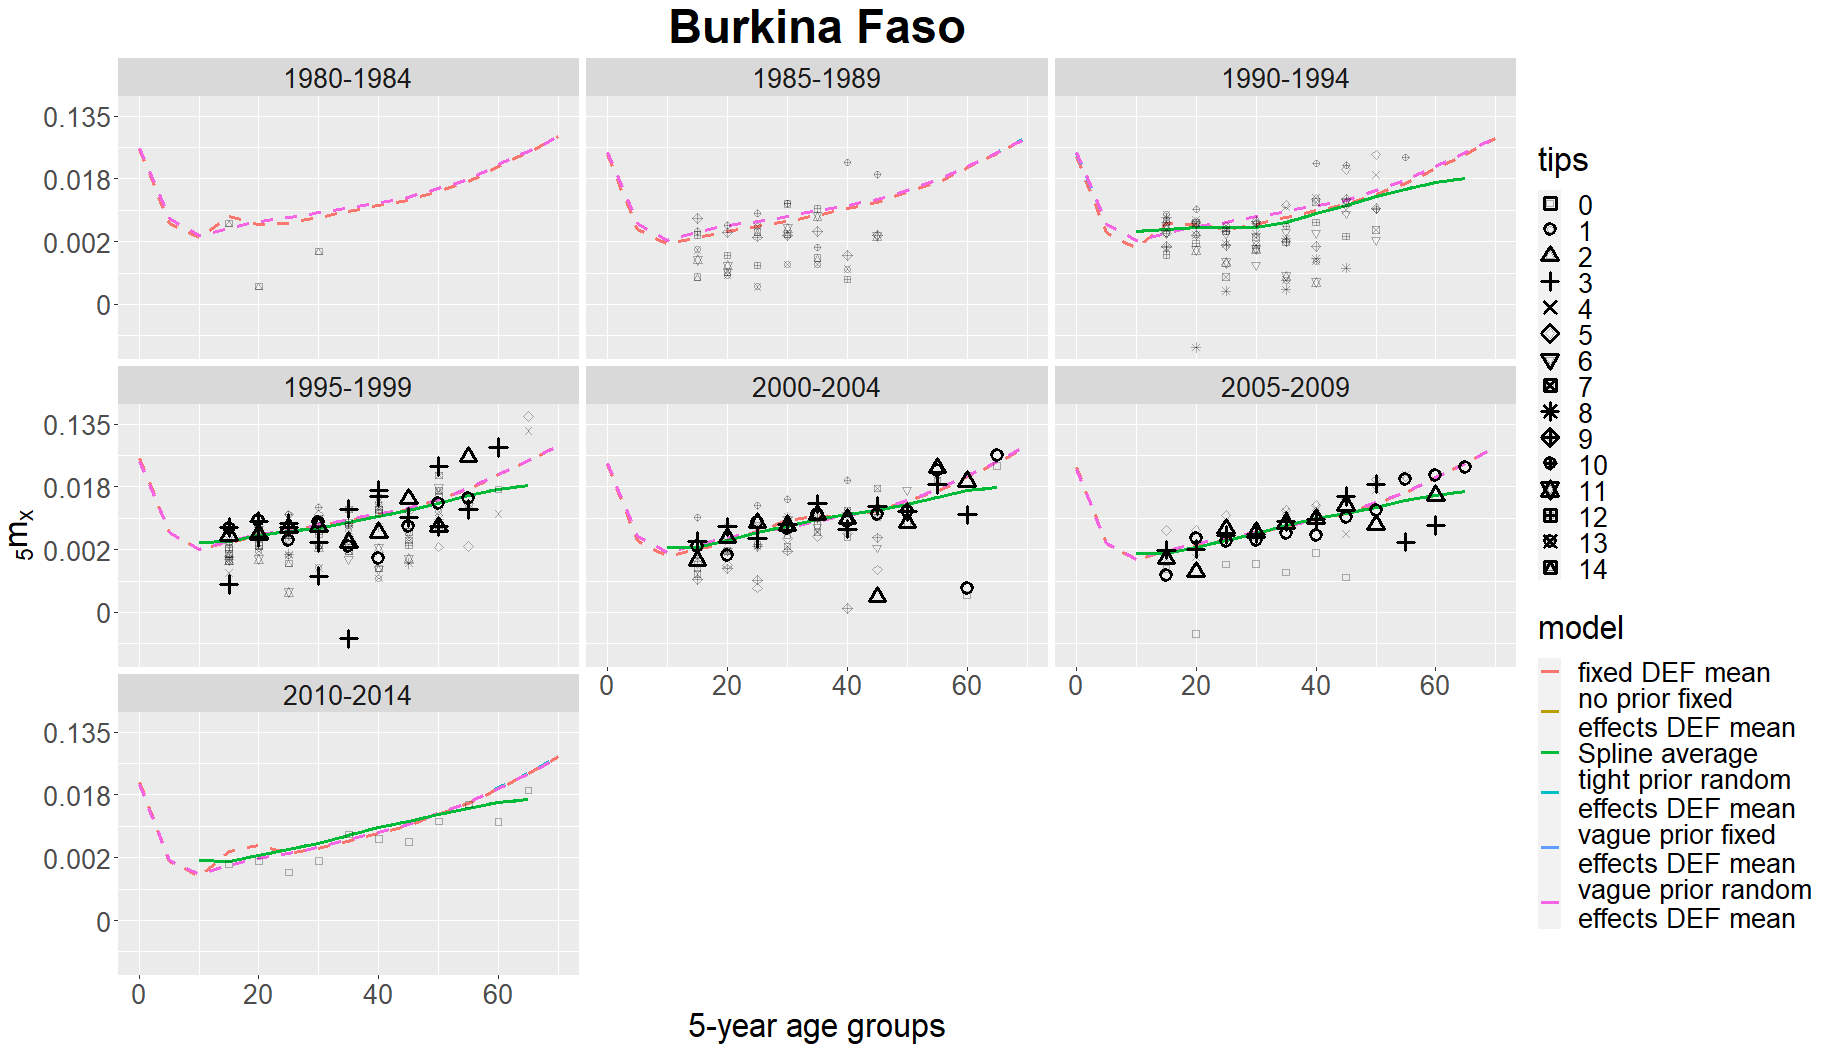
\includegraphics[width = \linewidth]{Burkina Faso/9/females LQDEF.png}
\end{figure}

\newpage
\section*{\centering Females LQ and DEF decomposed}
\begin{figure}[H]
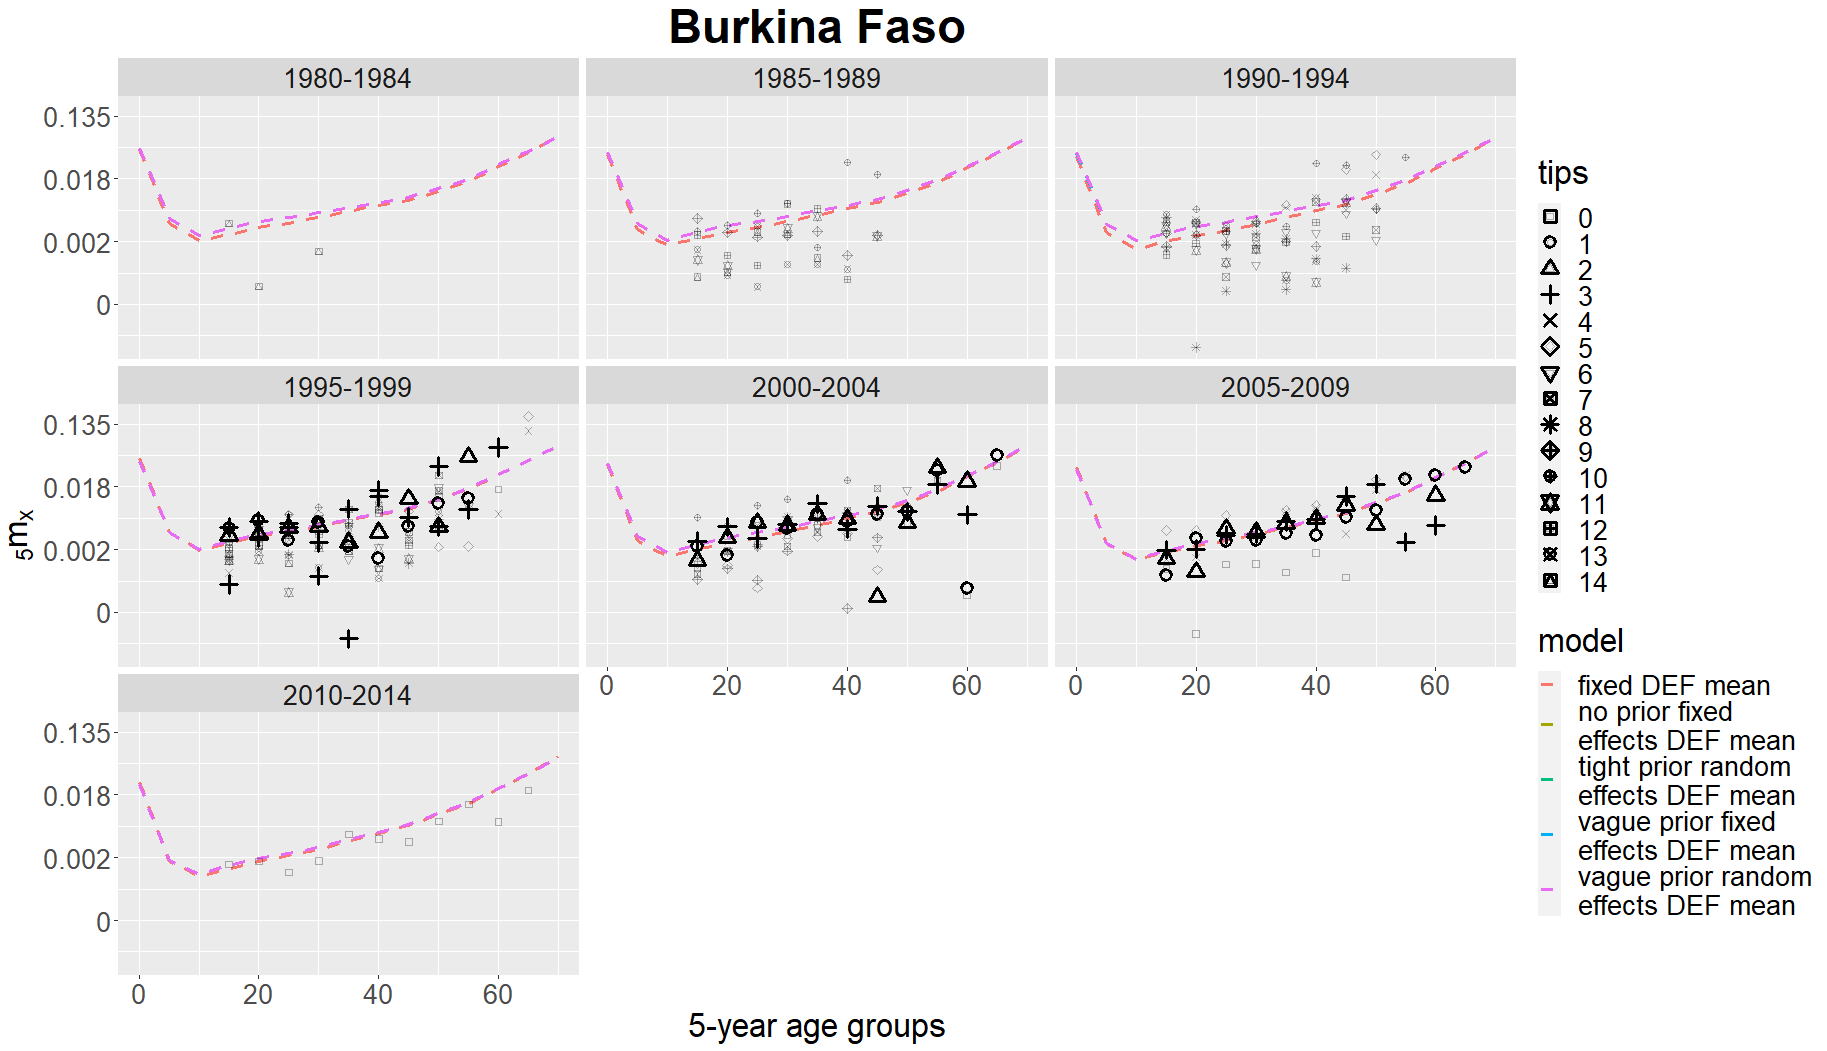
\includegraphics[width = \linewidth]{Burkina Faso/9/females LQ.png}
\end{figure}
\begin{figure}[H]
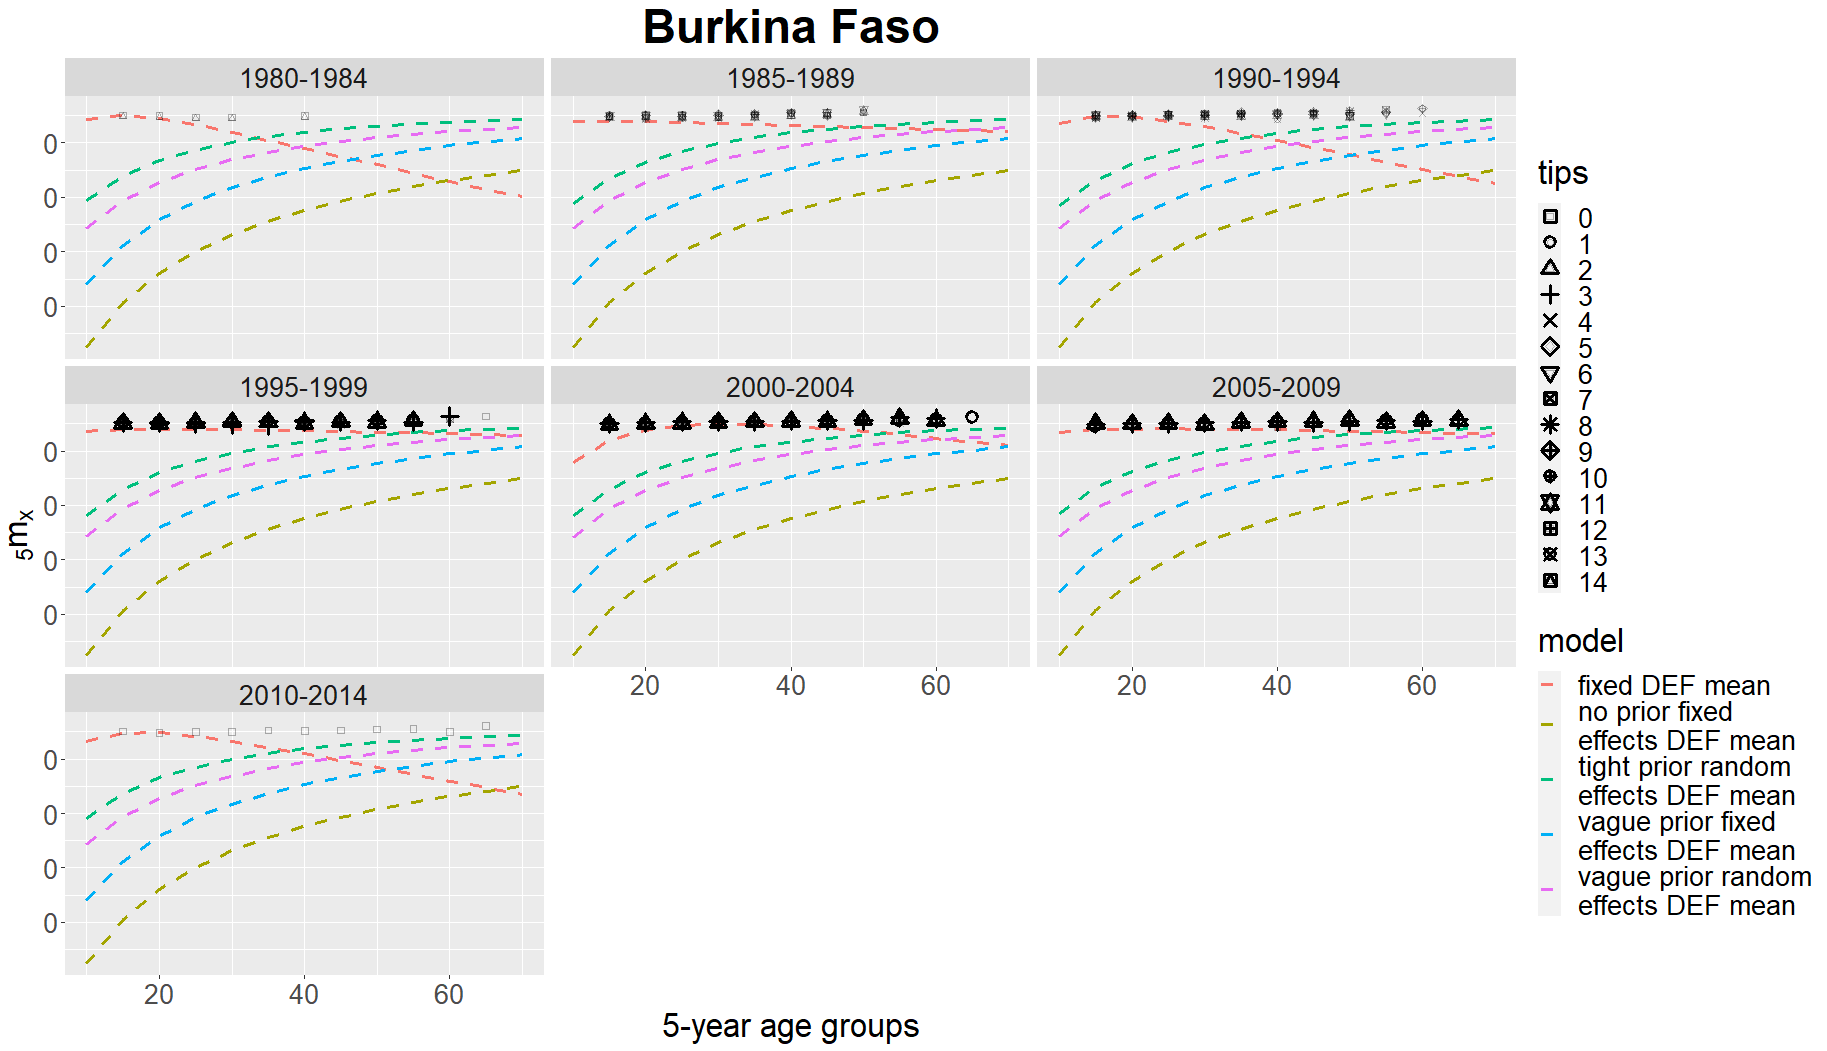
\includegraphics[width = \linewidth]{Burkina Faso/9/females DEF.png}
\end{figure}
\begin{itemize}
\item DEF peaks at crazy old ages in most cases
\end{itemize}

\newpage
\section*{\centering Males estimated mortality schedule}
\begin{figure}[H]
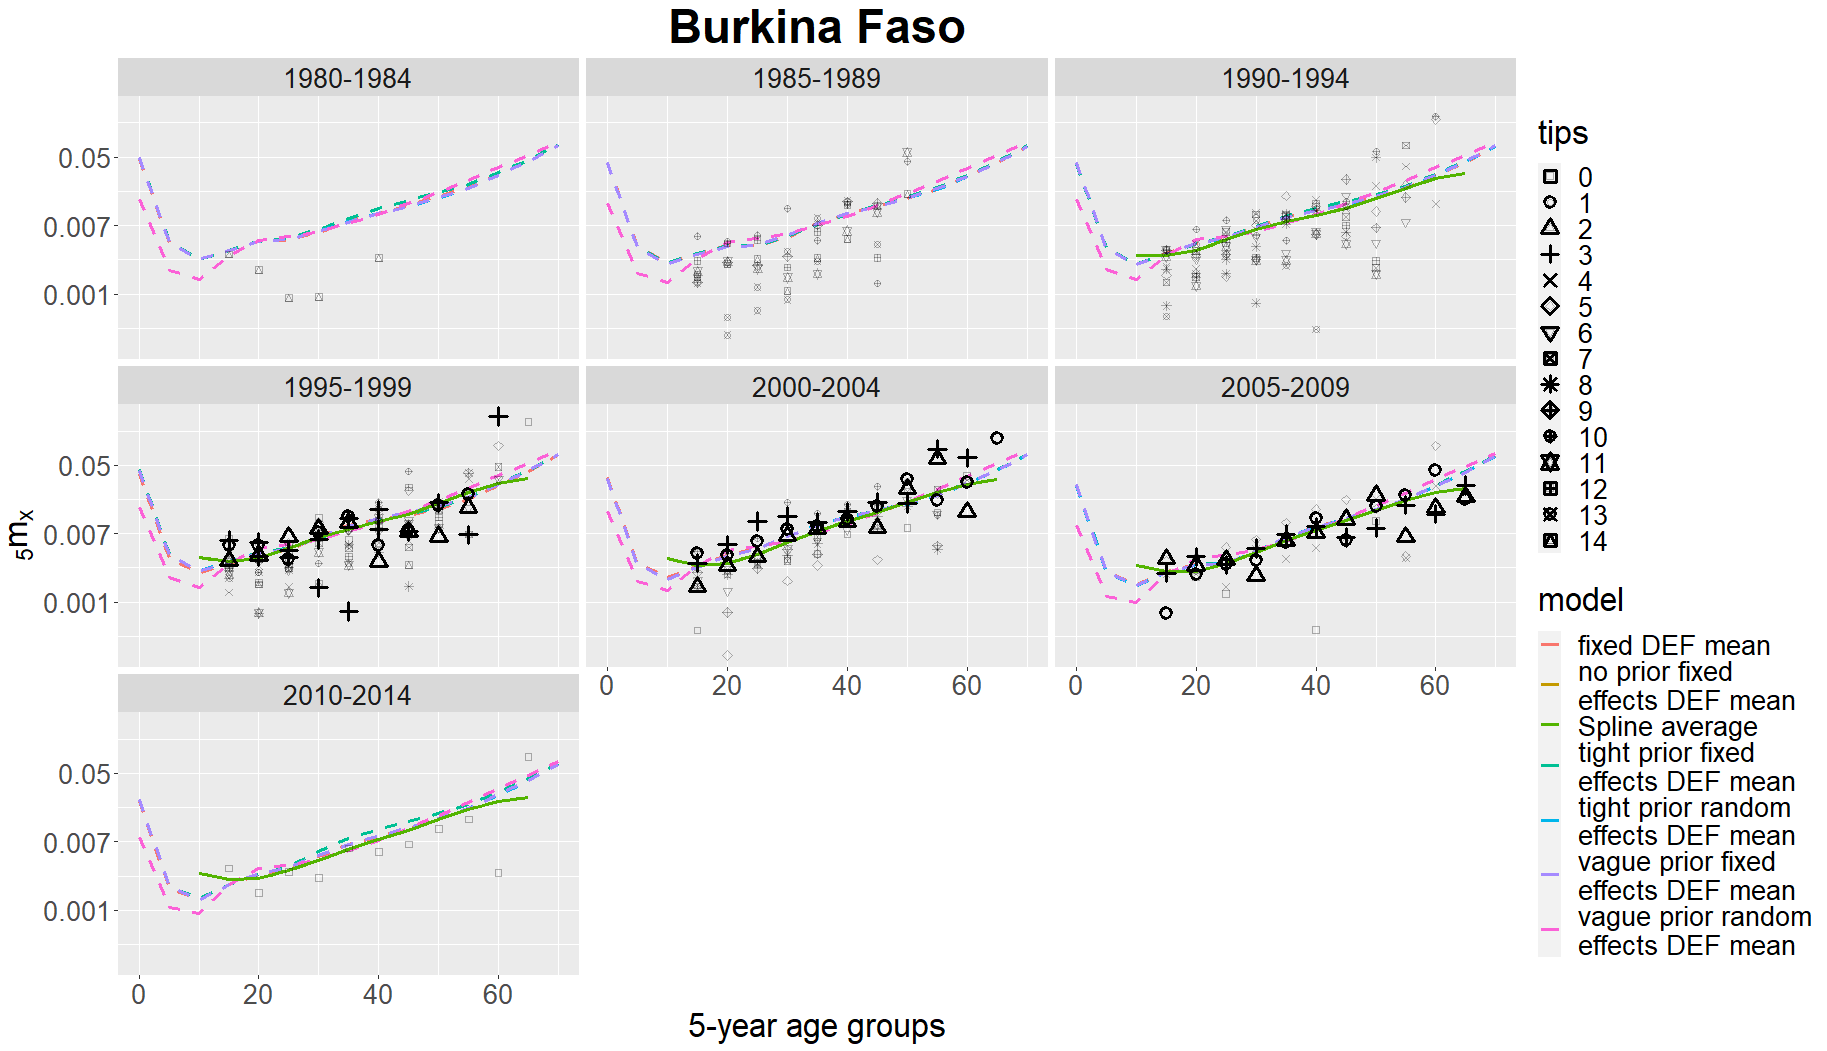
\includegraphics[width = \linewidth]{Burkina Faso/9/males LQDEF.png}
\end{figure}

\newpage
\section*{\centering Males LQ and DEF decomposed}
\begin{figure}[H]
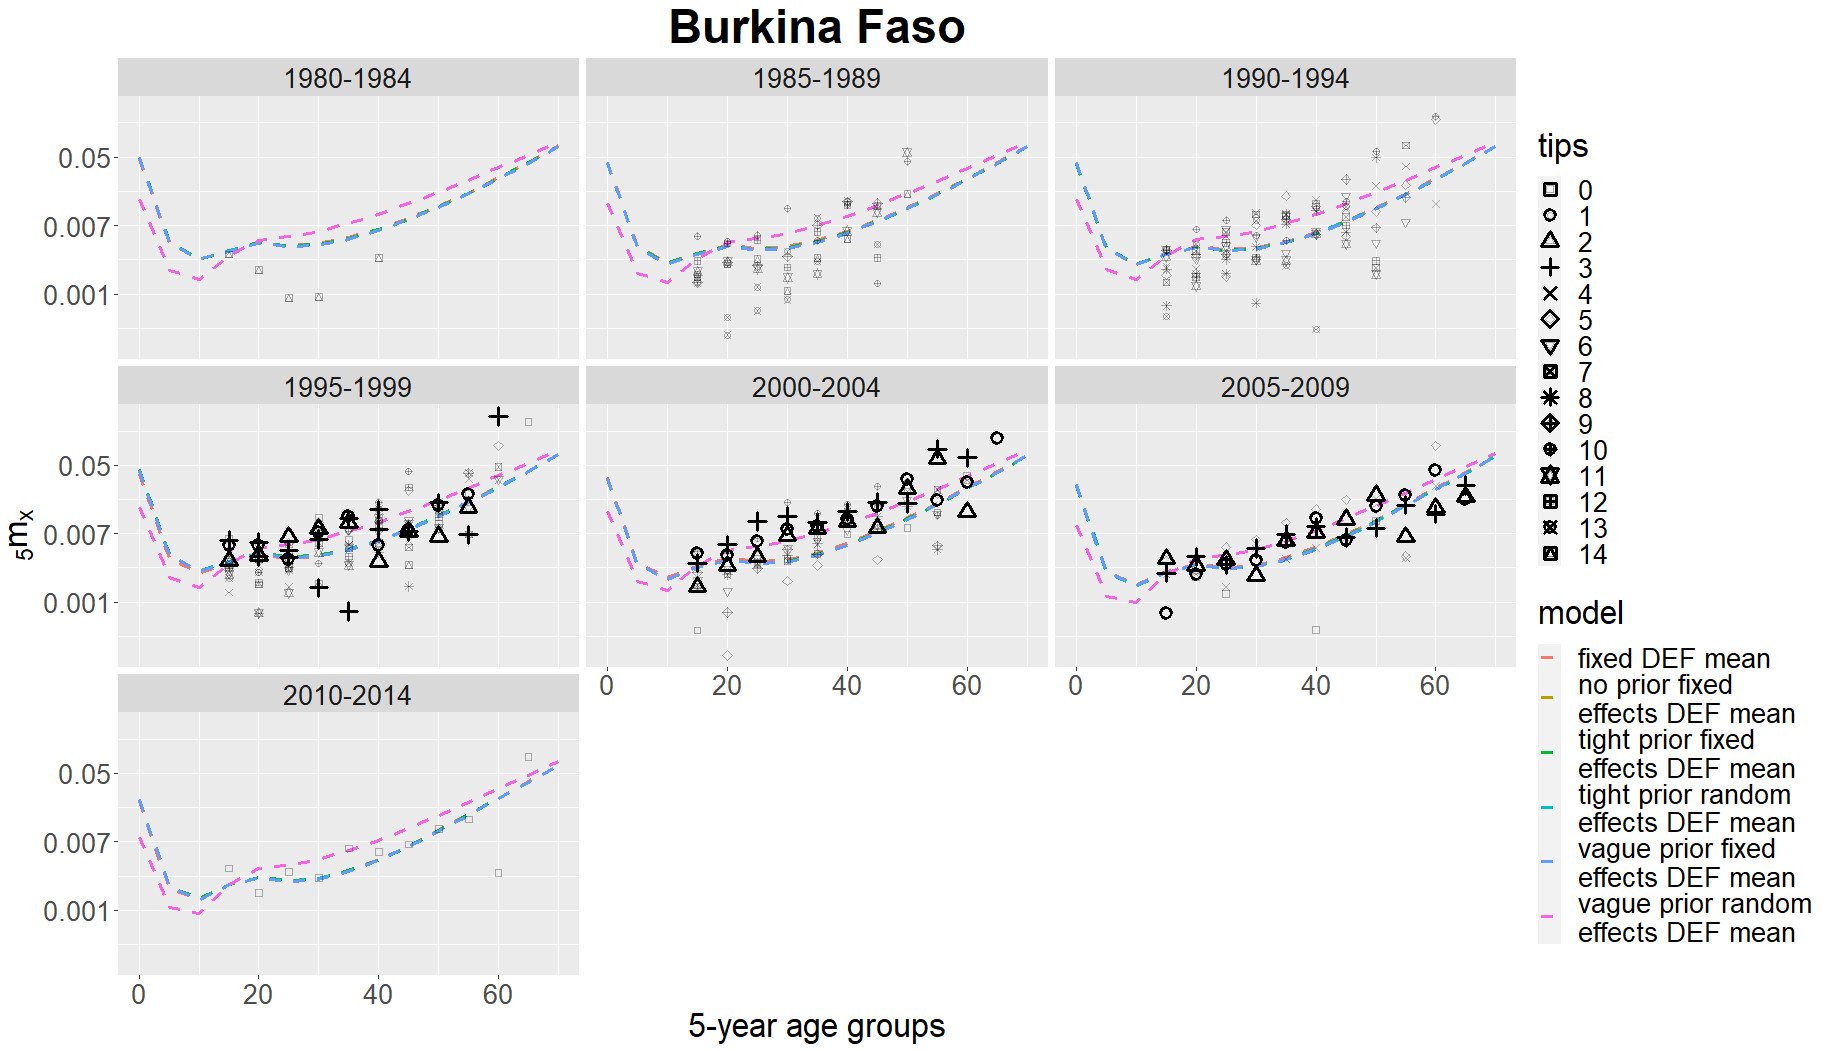
\includegraphics[width = \linewidth]{Burkina Faso/9/males LQ.png}
\end{figure}
\begin{figure}[H]
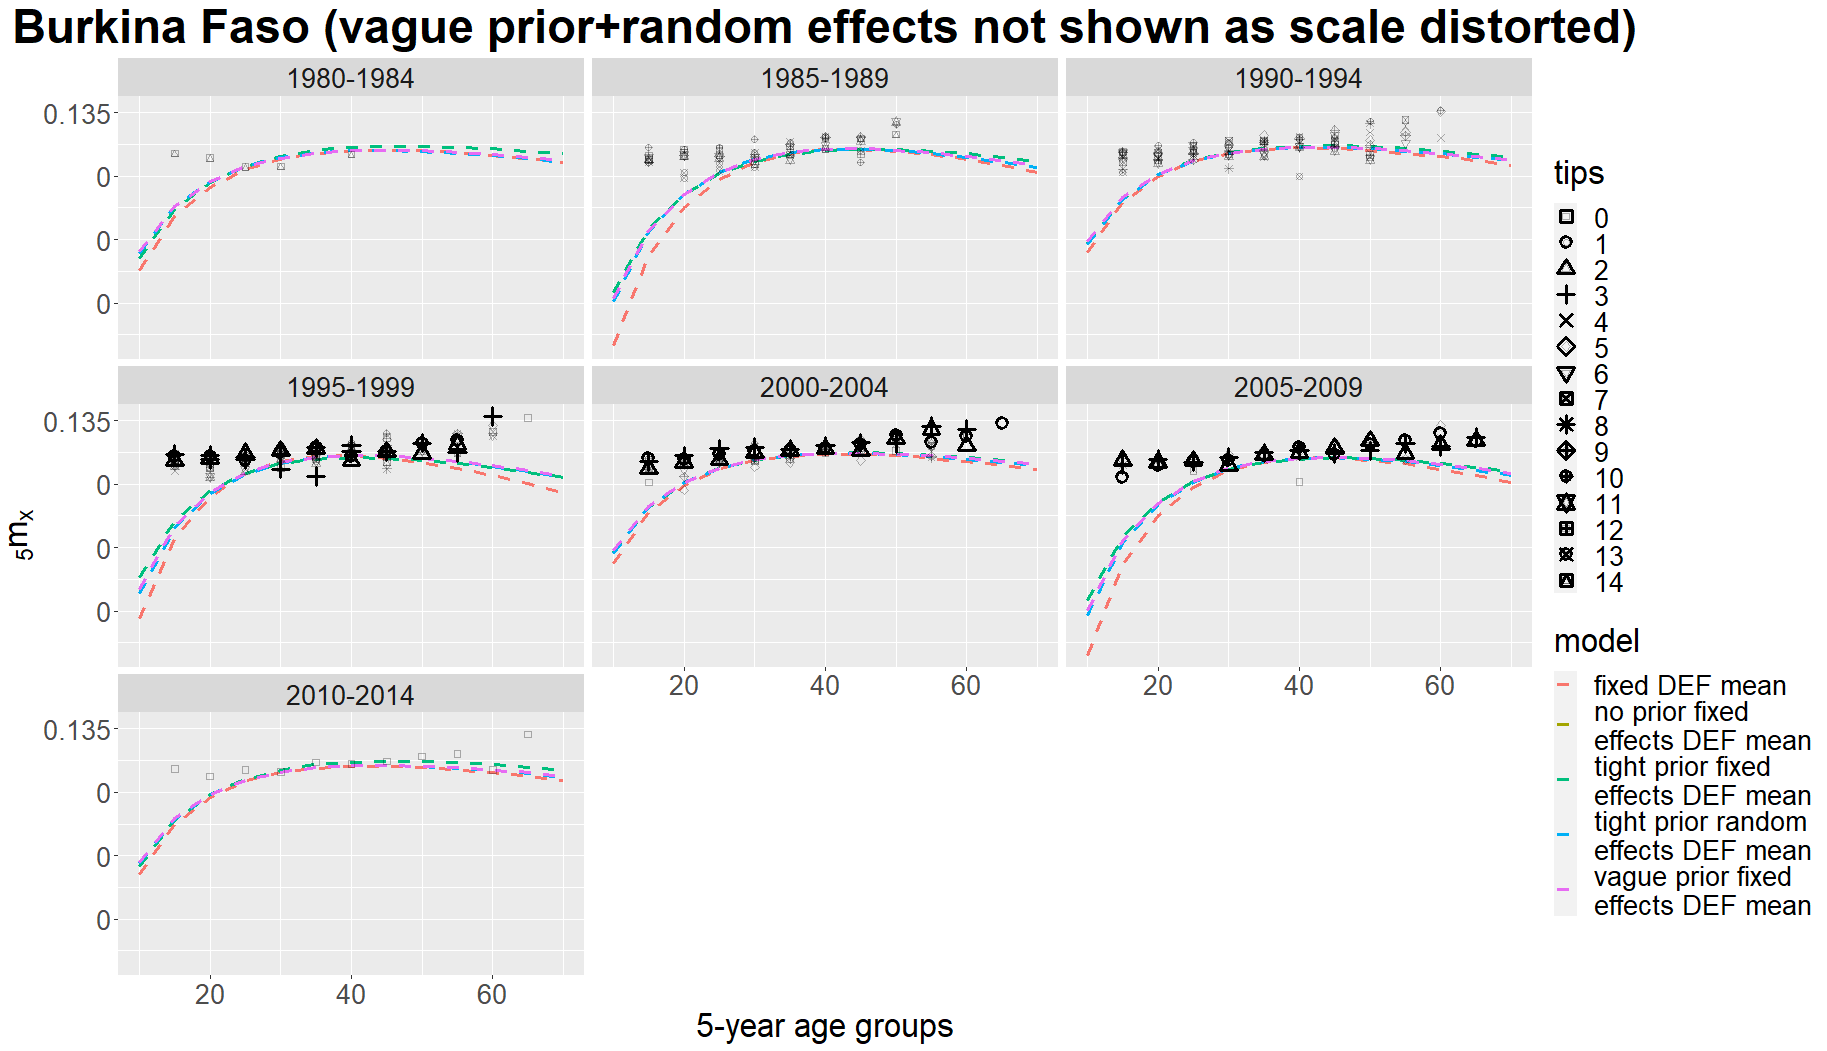
\includegraphics[width = \linewidth]{Burkina Faso/9/males DEF.png}
\end{figure}
\begin{itemize}
\item DEF peaks at around age 45 in most cases, except when $\mu_i$ are given vague priors and treated as random effects
\end{itemize}
 
\newpage
\begin{itemize}
\item Tried to fit the Thiele model which has the following form:
 \begin{align*}
m(x) = \underbrace{\varphi e^{-\psi x}}_\text{negative exponential} + \, \underbrace{\lambda e^{-\delta (\textcolor{red}{x}-\textcolor{red}{\epsilon})^2}}_\text{normal}+ \underbrace{A e^{B x}}_\text{Gompertz} \qquad \varphi,\psi,\lambda,\delta,\epsilon > 0
 \end{align*}
compared to the HP-8 model:
 \begin{align*}
\frac{q_x}{1-q_x} = A^{(x + B)^C} + D e^{-E(\textcolor{red}{ln x} - \textcolor{red}{ln F})^2} + GH^x
 \end{align*}
  \begin{itemize}
	\item[--] modelled on $m_x$ directly
	\item[--] 7 parameters
	\item[--] priors for the parameters of the Thiele model are obtained by regressing the model on the mortality schedules from the LogQuad models fixing $h$ at IGME estimates and $k = 0$ 
	\begin{itemize}
	\item[1)] set age $=$ seq(2, 92, by = 5)
	\item[2)] regressed $\varphi e^{-\psi x}$ on LogQuad $m_x$ from age $0$-$4$ to $10$-$14$, with penalties such that $m_0$ is consistent with the mortality rate implied by the IGME estimates
	\item[3)] regressed $\lambda e^{-\delta (x-\epsilon)^2}$ on Logquad $m_x$ from age $10$-$14$ to $40$-$44$
	\item[4)] regressed $A e^{B x}$ on LogQuad $m_x$ from age $65$-$69$ to $90$-$94$
	\item[5)] regressed the whole model $\varphi e^{-\psi x} + \lambda e^{-\delta (x-\epsilon)^2} + A e^{B x}$ on LogQuad $m_x$ from age 0-4 to age 90-94, with penalties such that estimated $m_0$ are close the IGME implied levels
	\end{itemize}
	\item[--] all parameters are given log-normal priors with the regressed values as prior means and standard deviation $\sigma_i \sim IG(1, 0.01)$
	\item[--] the estimated hump seems to still have quite a strong influence at the youngest ages relative to the mid ages, should I use $(\textcolor{red}{ln x} - \textcolor{red}{ln \epsilon})^2$ as in the HP-8 model for the hump in Thiele?
	\end{itemize}
\item Initial values when fitting to males sometimes need a bit tweaking (but still easier then LQ + DEF in my experience), especially the precision parameters, or maybe I was just lucky with females
\item Modelled all parameters as AR(1) processes around the prior means, yet to check the estimated $\rho_i$
\item Have done a simple robustness test on $\epsilon$ by setting different prior means manually
\end{itemize}

\newpage
\section*{\centering Females estimated mortality schedules}
\begin{figure}[H]
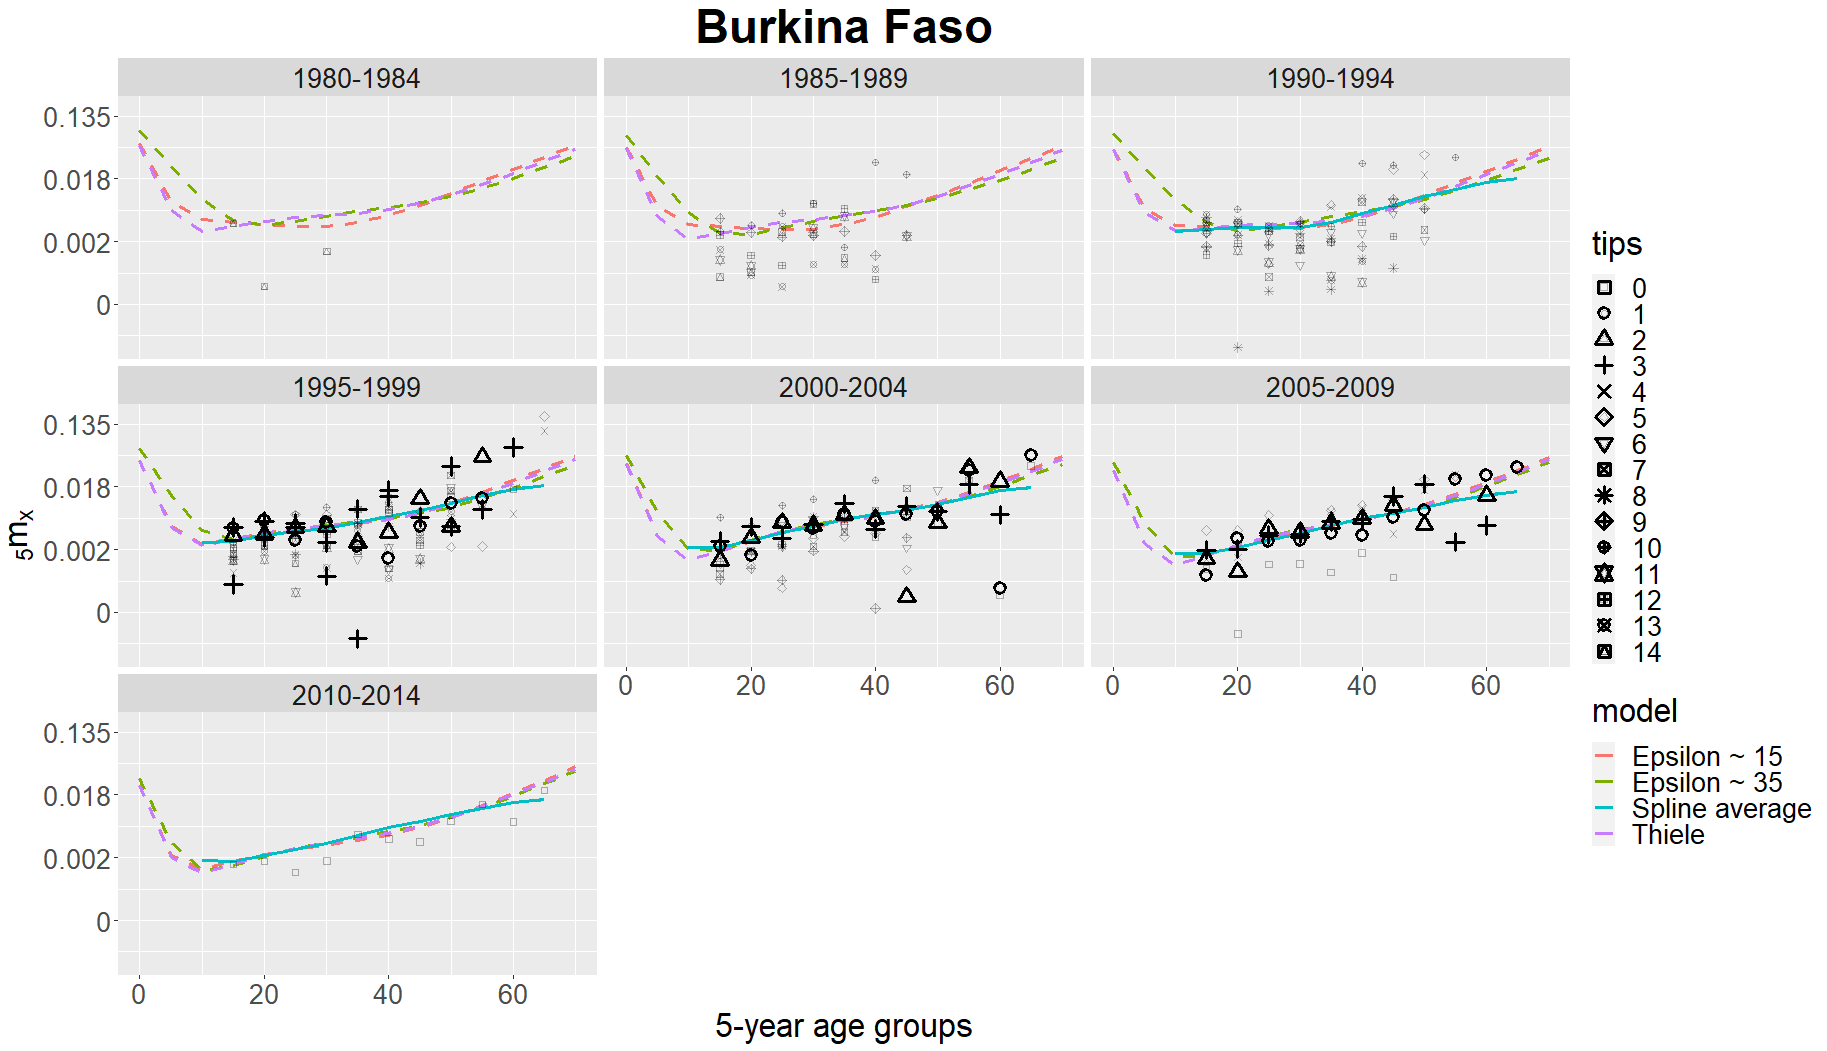
\includegraphics[width = \linewidth]{Burkina Faso/9/Thiele female.png}
\end{figure}
\begin{figure}[H]
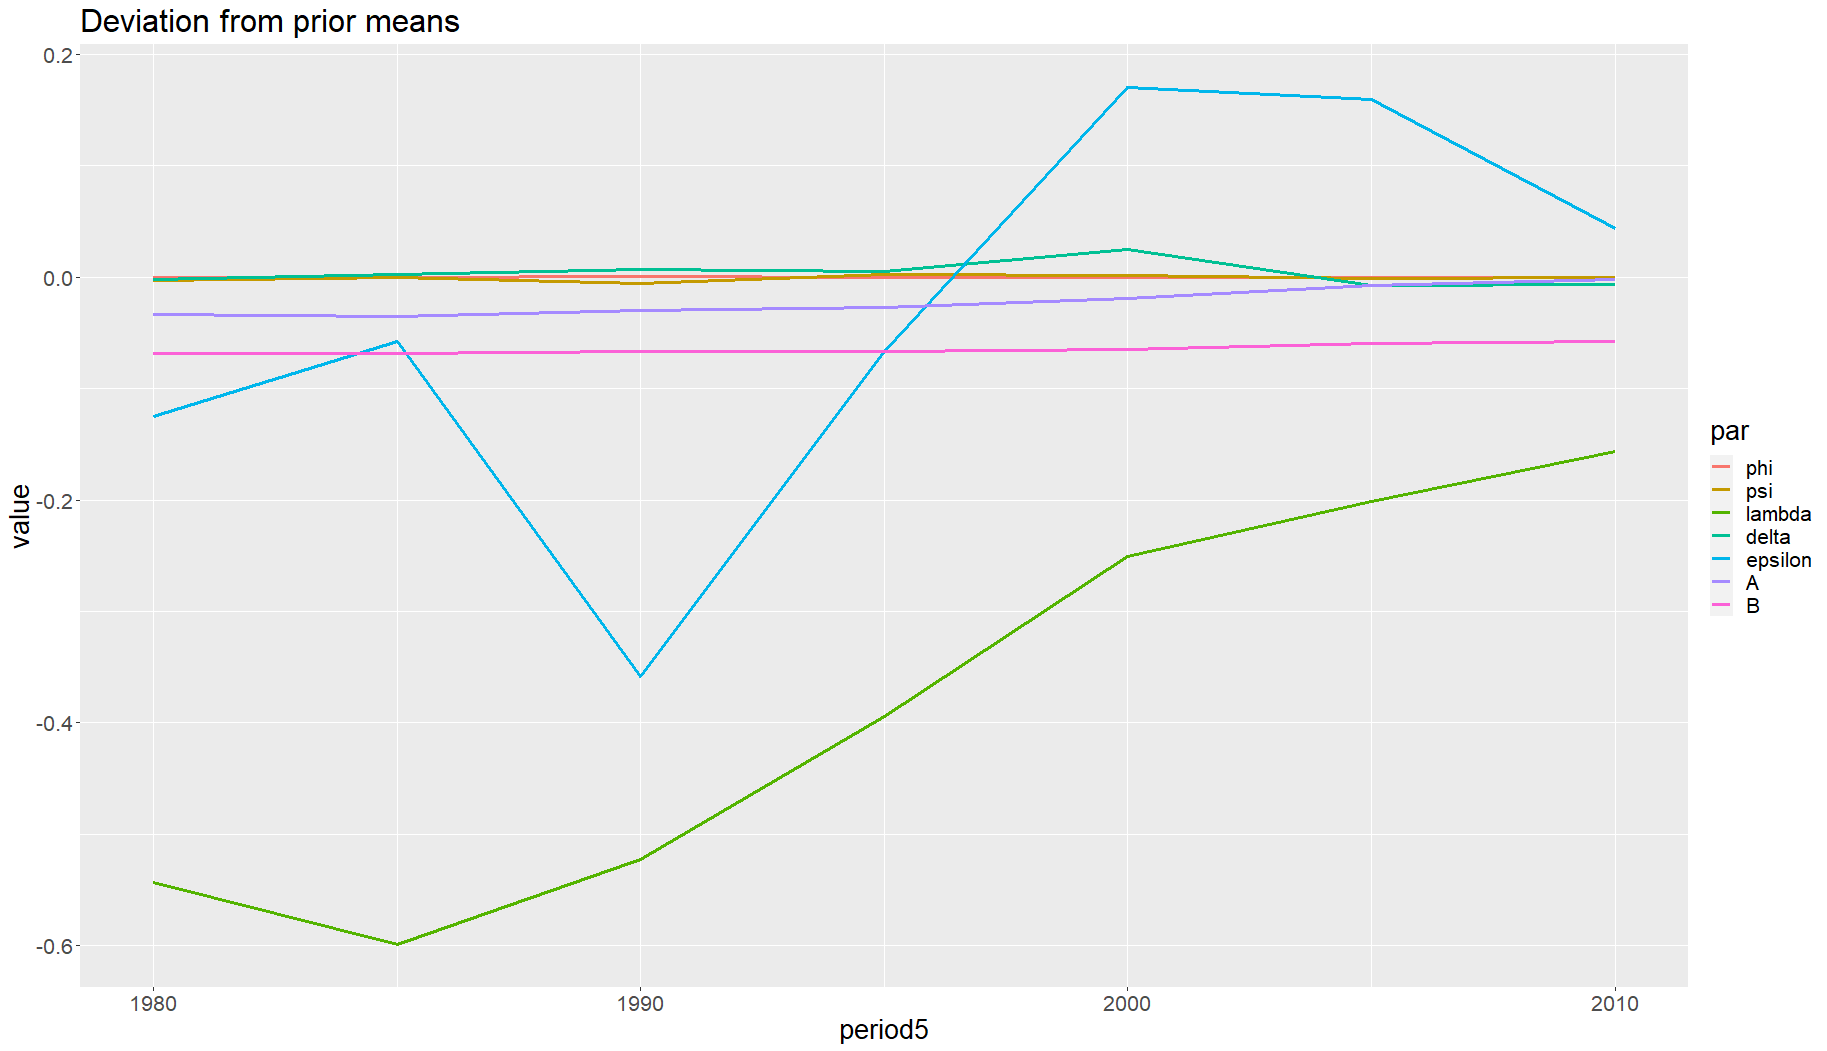
\includegraphics[width = \linewidth]{Burkina Faso/9/Thiele female par deviation.png}
\end{figure}
\begin{itemize}
\item most variations seen in $\lambda$ and $\epsilon$
\end{itemize}


\newpage
\section*{\centering Females Thiele Decomposed}
\begin{figure}[H]
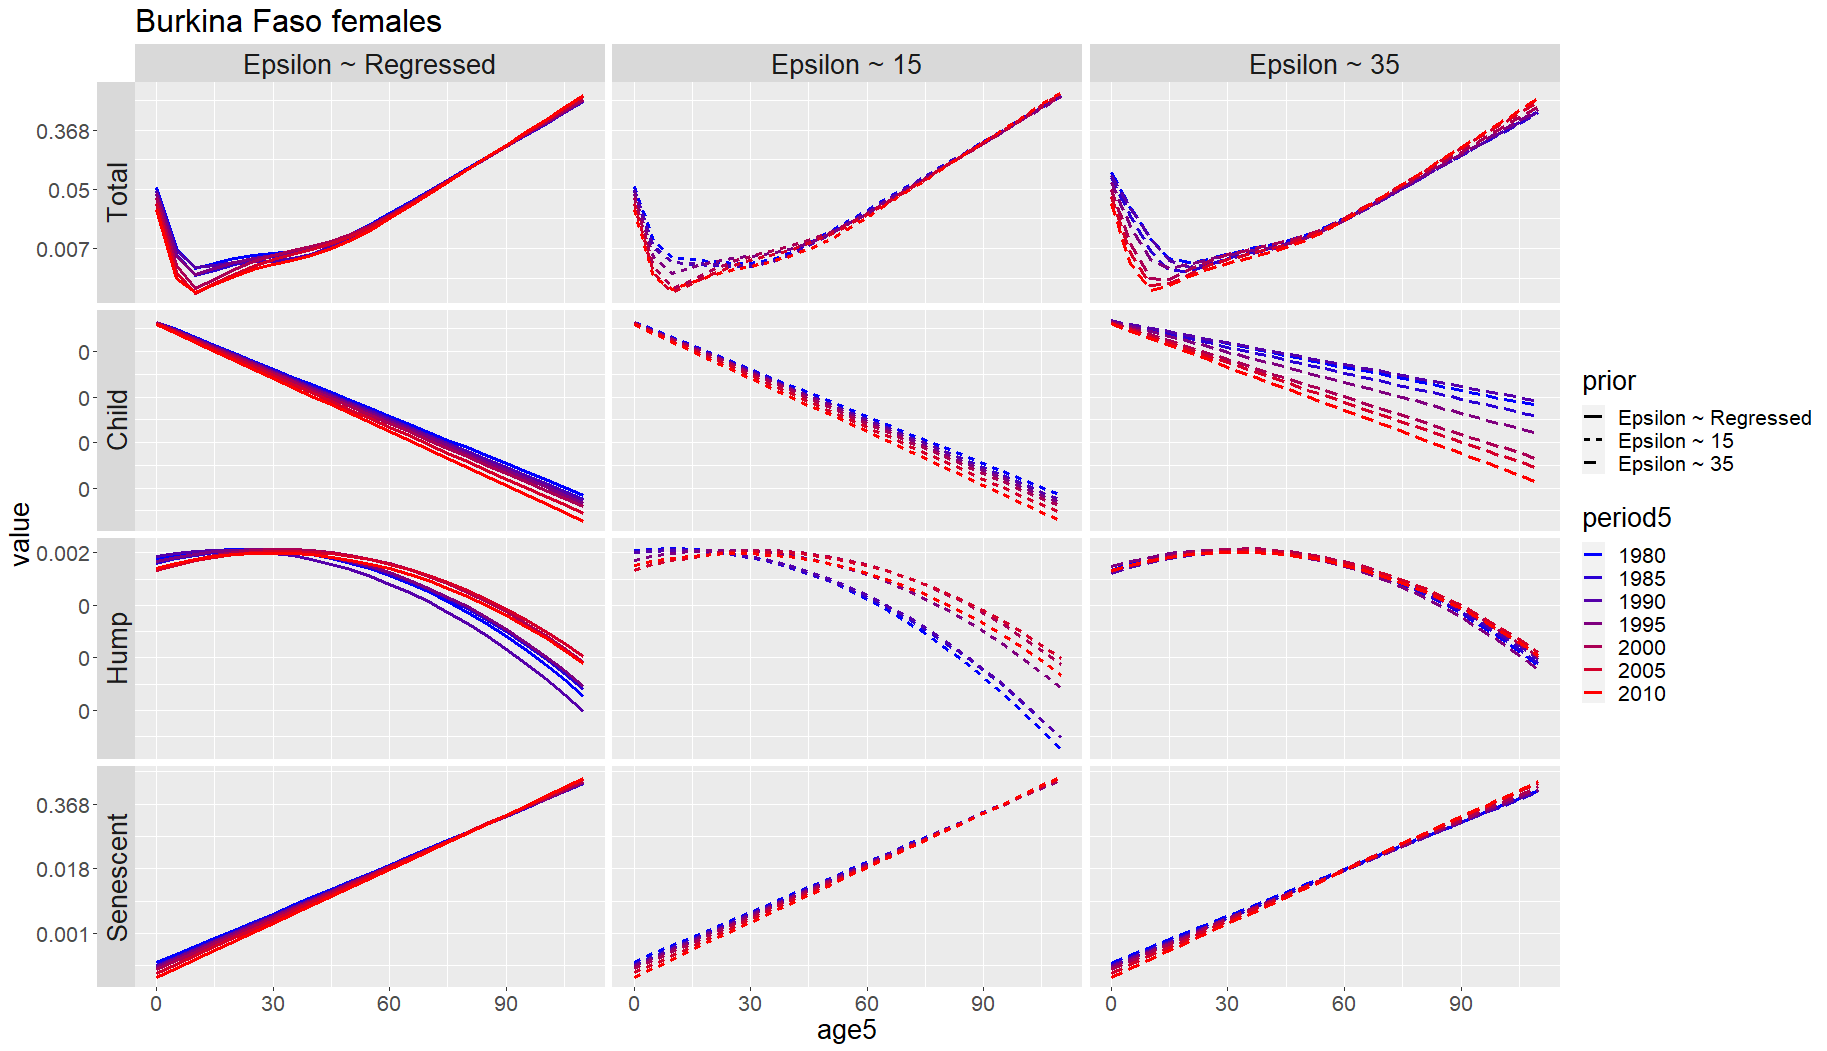
\includegraphics[width = \linewidth]{Burkina Faso/9/Thiele female decomp.png}
\end{figure}
\begin{itemize}
\item slight shift in estimated $\epsilon$ to older ages
\item when prior means for $\epsilon$ set to 35 doesnt seem to shift
\end{itemize}

\newpage
\section*{\centering Males estimated mortality schedules}
\begin{figure}[H]
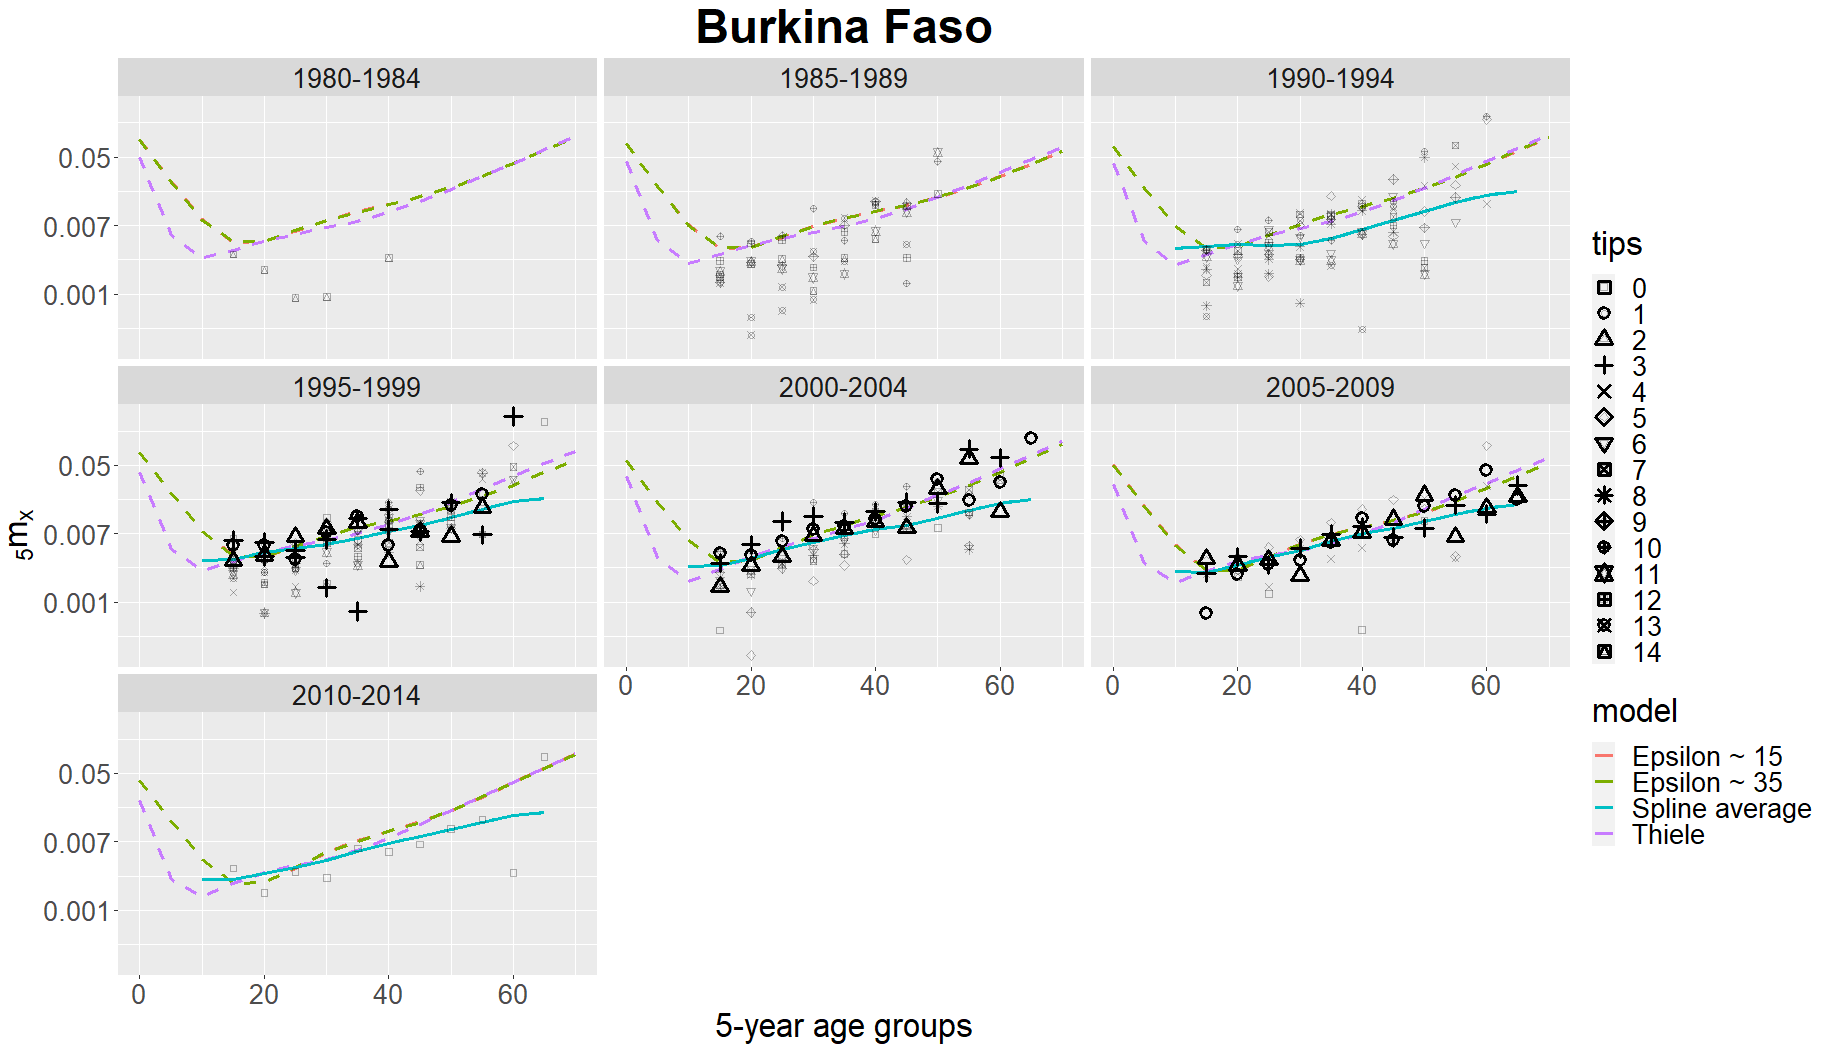
\includegraphics[width = \linewidth]{Burkina Faso/9/Thiele male.png}
\end{figure}
\begin{figure}[H]
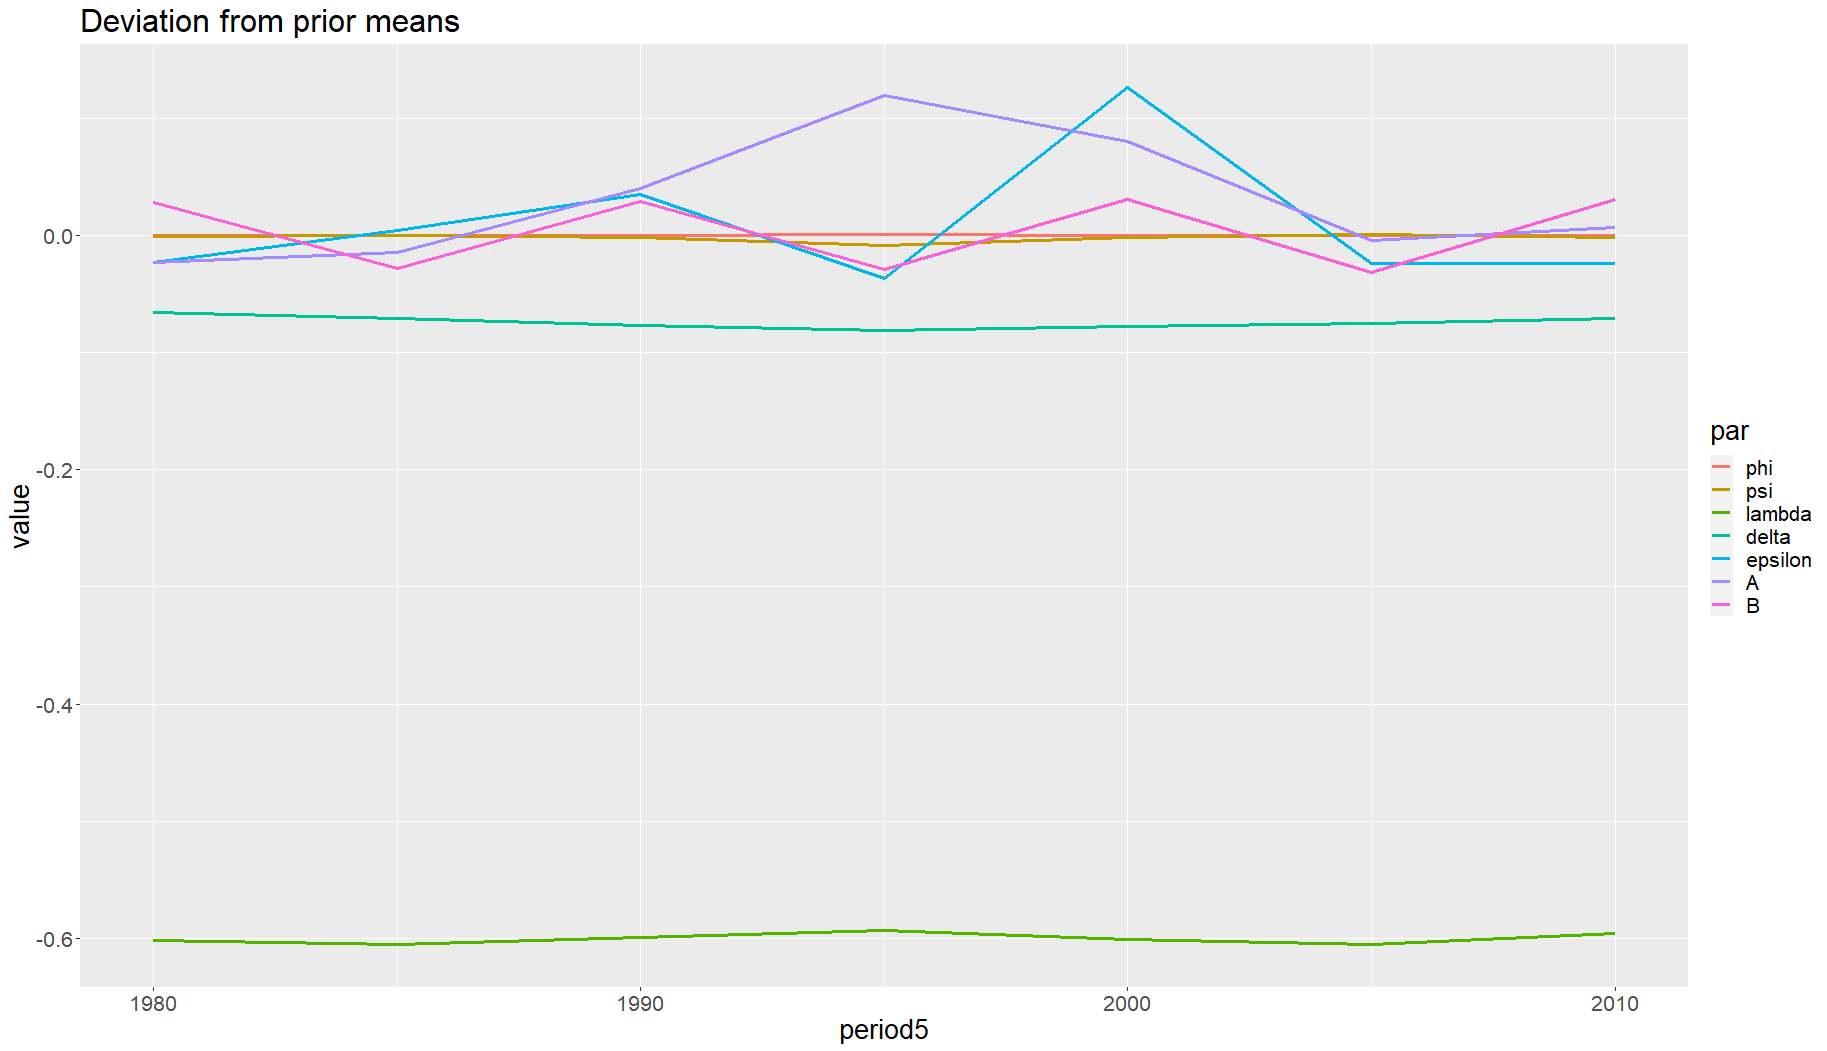
\includegraphics[width = \linewidth]{Burkina Faso/9/Thiele male par deviation.png}
\end{figure}
\begin{itemize}
\item most variations seen in $\lambda$
\end{itemize}


\newpage
\section*{\centering Males Thiele Decomposed}
\begin{figure}[H]
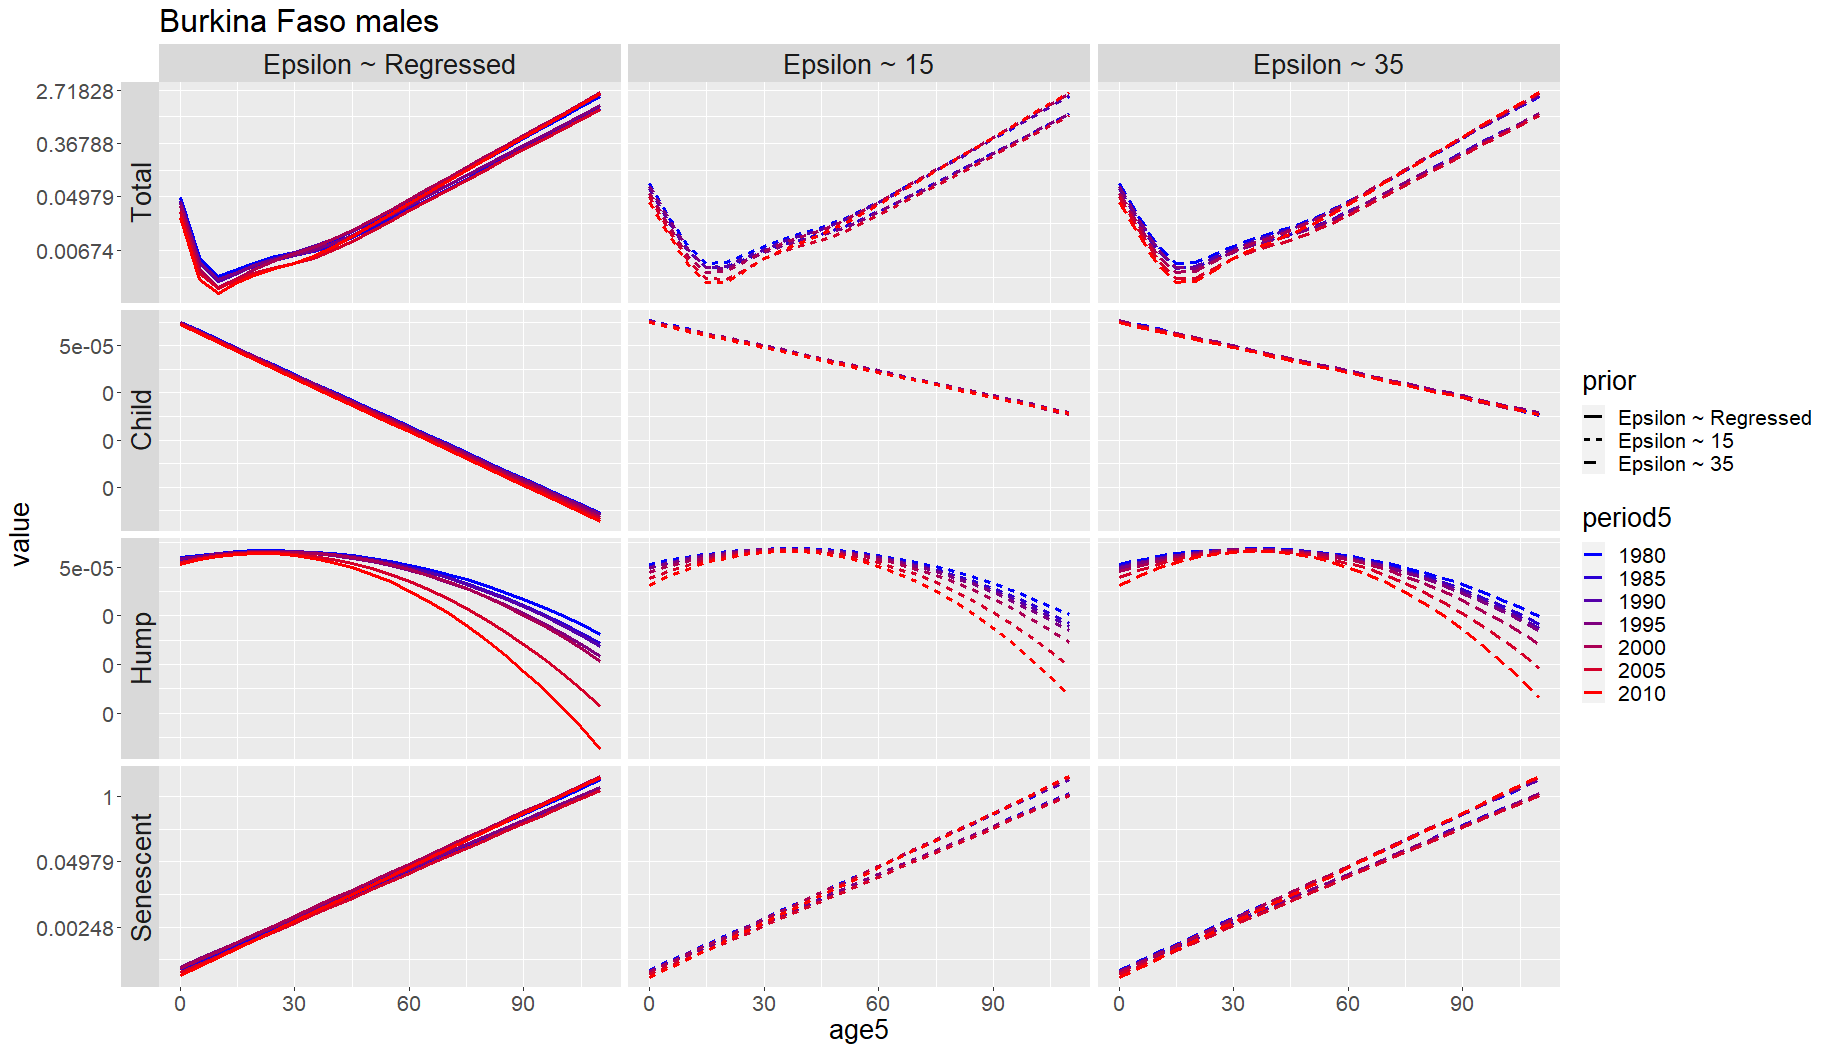
\includegraphics[width = \linewidth]{Burkina Faso/9/Thiele male decomp.png}
\end{figure}
\begin{itemize}
\item slight shift in estimated $\epsilon$ to \textcolor{red}{younger} ages (whereas in females it moves to older ages)
\item seem to be more robust for males as the shapes are more consistent even with different prior means on $\epsilon$, possibly because of a more identifiable hump?
\item \textcolor{red}{Female spline estimates plotted by mistake!}
\end{itemize}

\newpage
\section*{Also tried to fit to some selected countries}
\begin{figure}[H]
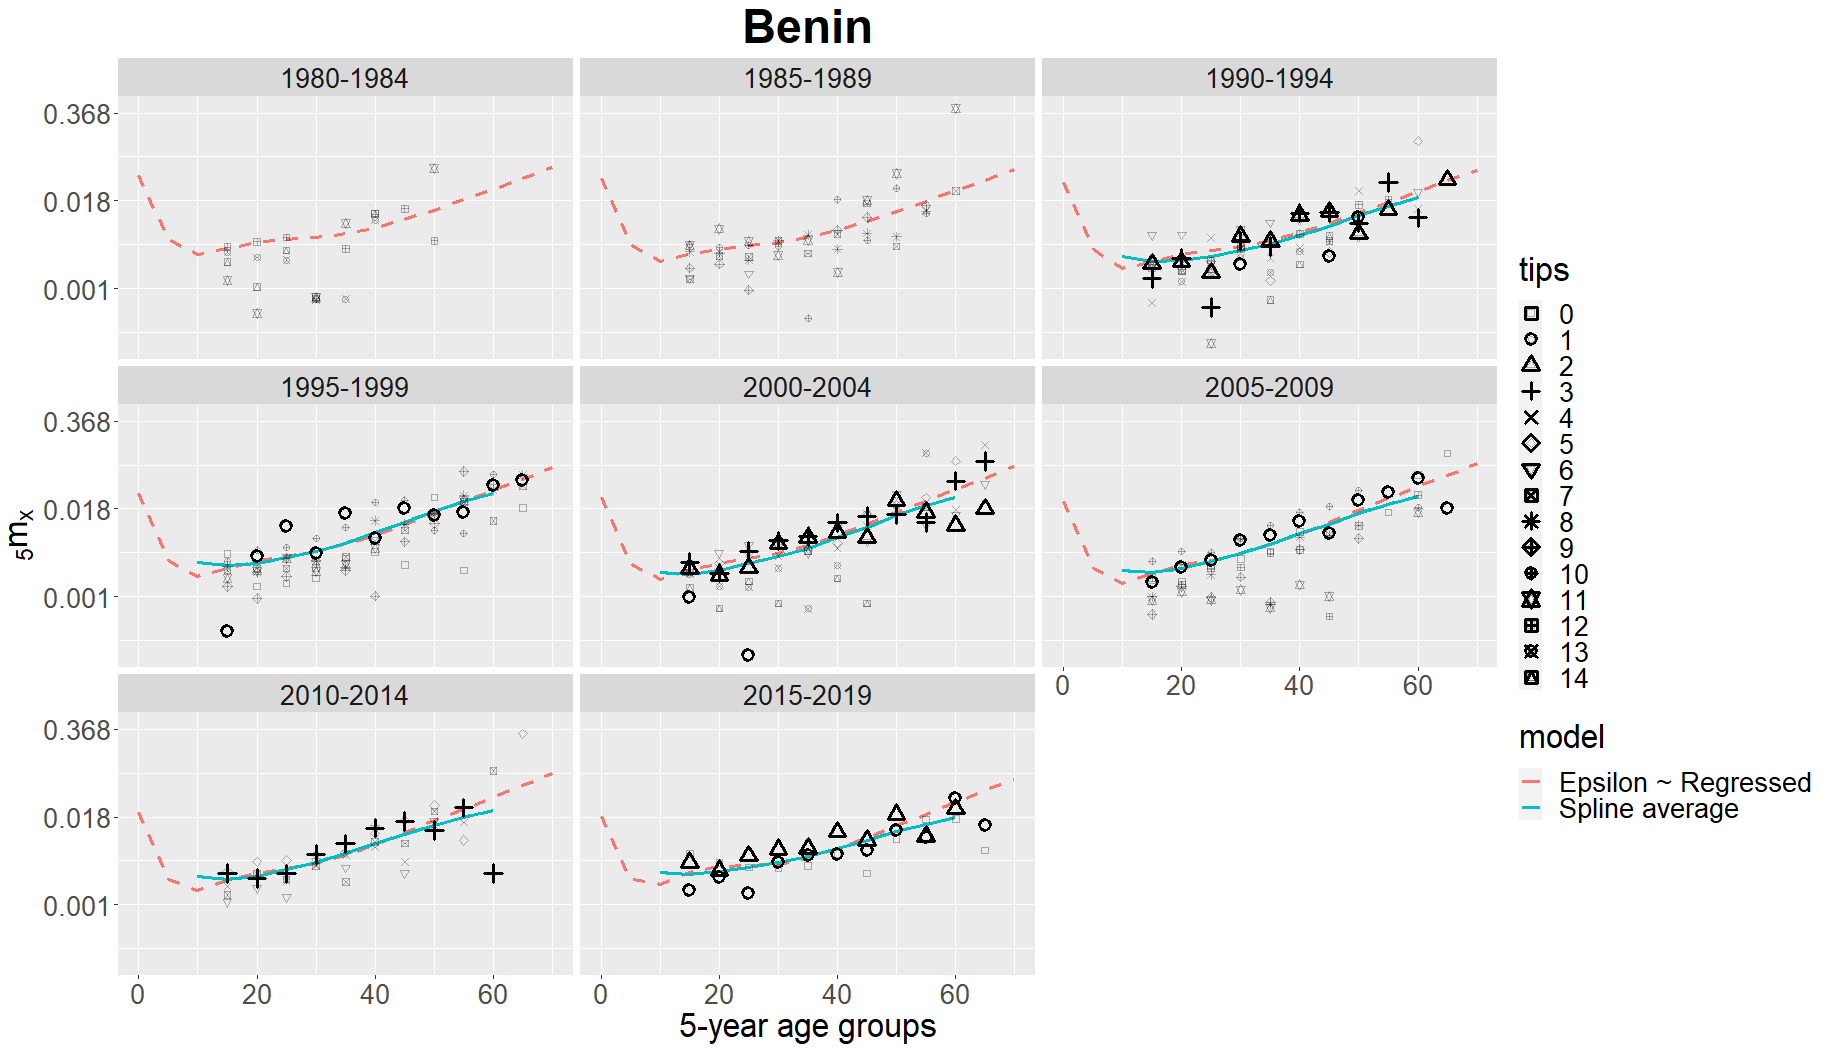
\includegraphics[width = \linewidth]{Burkina Faso/9/Benin male.png}
\caption*{Males}
\end{figure}
\begin{figure}[H]
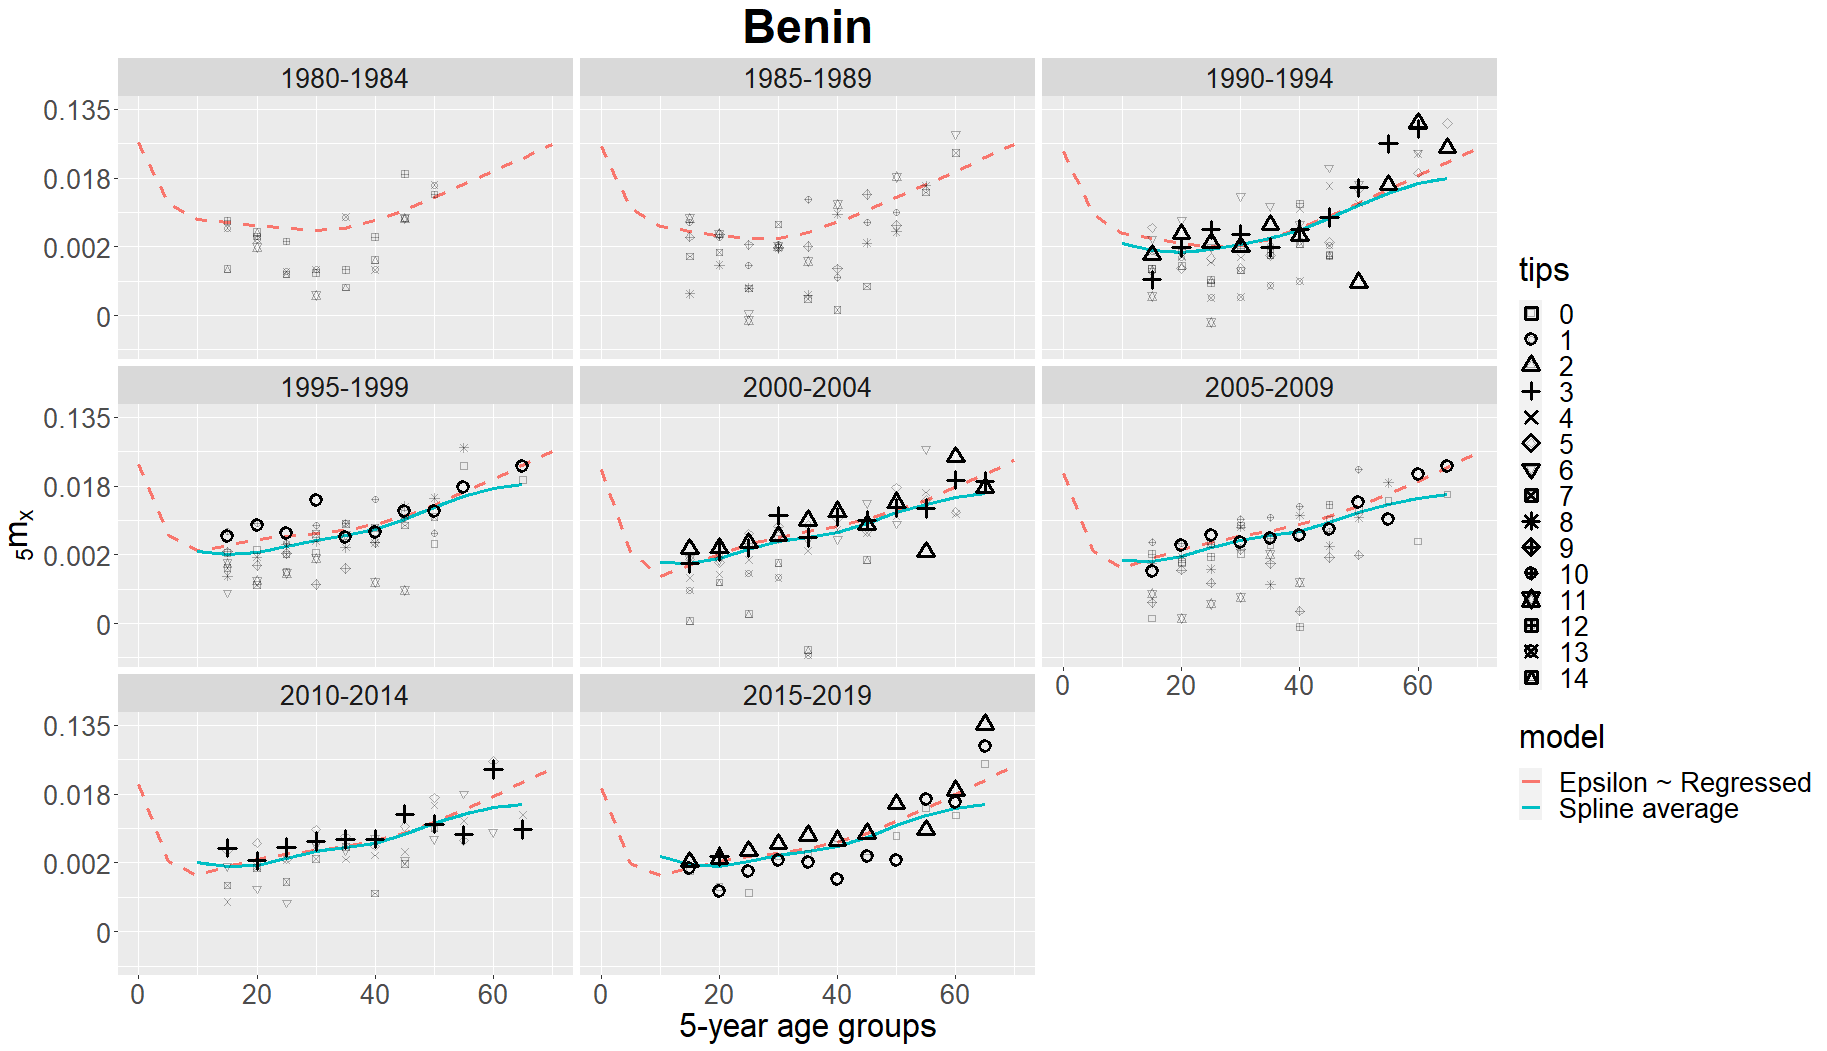
\includegraphics[width = \linewidth]{Burkina Faso/9/Benin female.png}
\caption*{Females}
\end{figure}

\newpage
\begin{figure}[H]
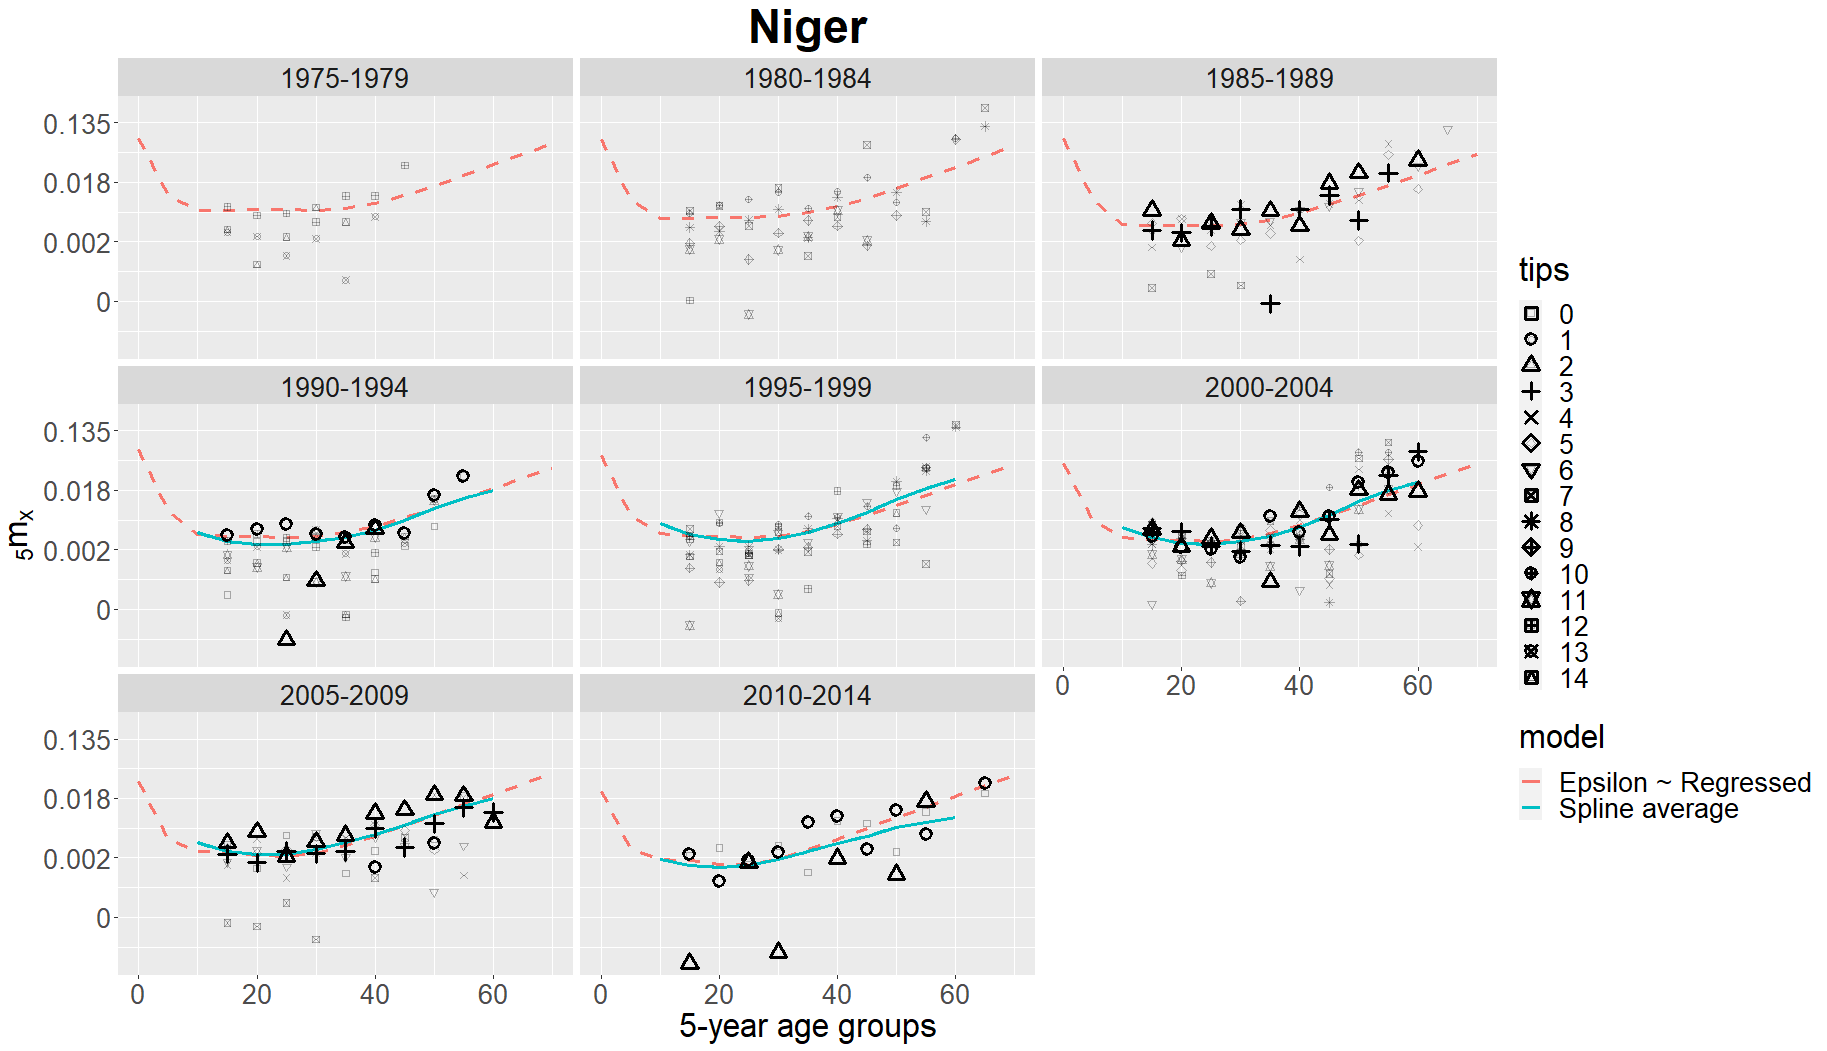
\includegraphics[width = \linewidth]{Burkina Faso/9/Niger male.png}
\caption*{Males}
\end{figure}
\begin{figure}[H]
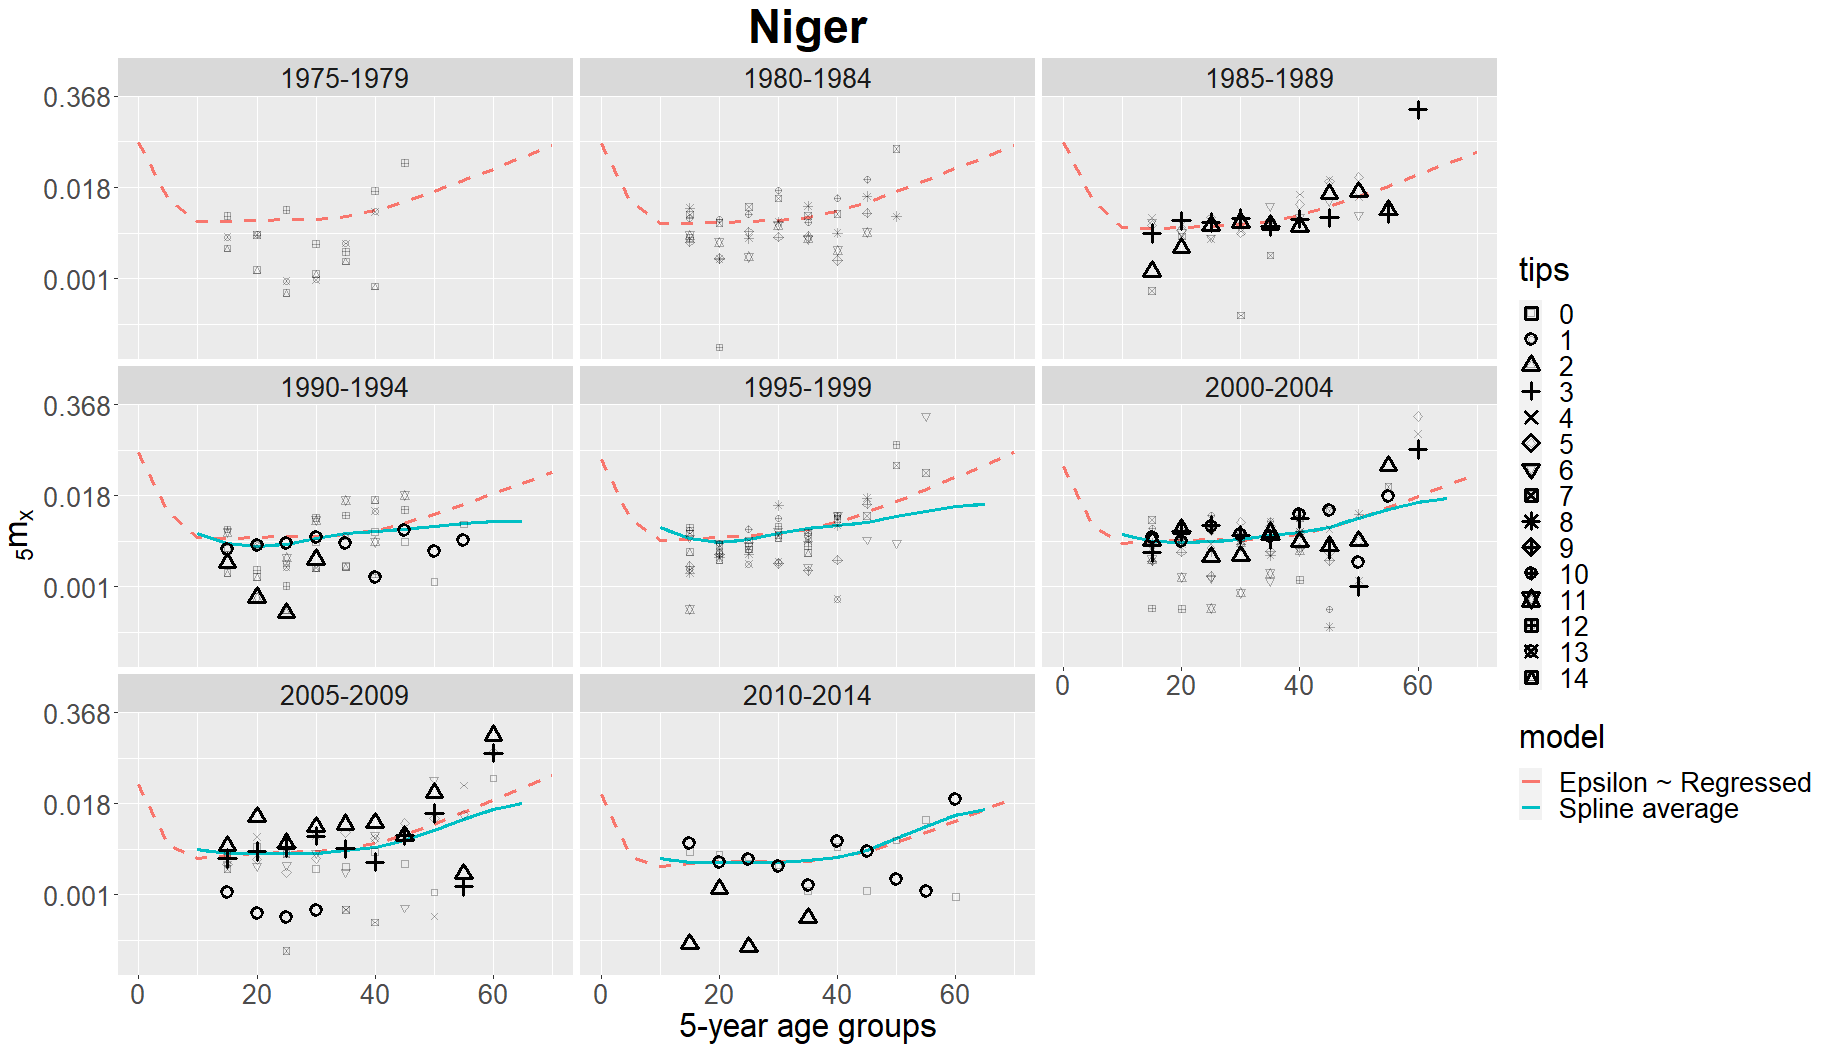
\includegraphics[width = \linewidth]{Burkina Faso/9/Niger female.png}
\caption*{Females}
\end{figure}

 \newpage
\begin{figure}[H]
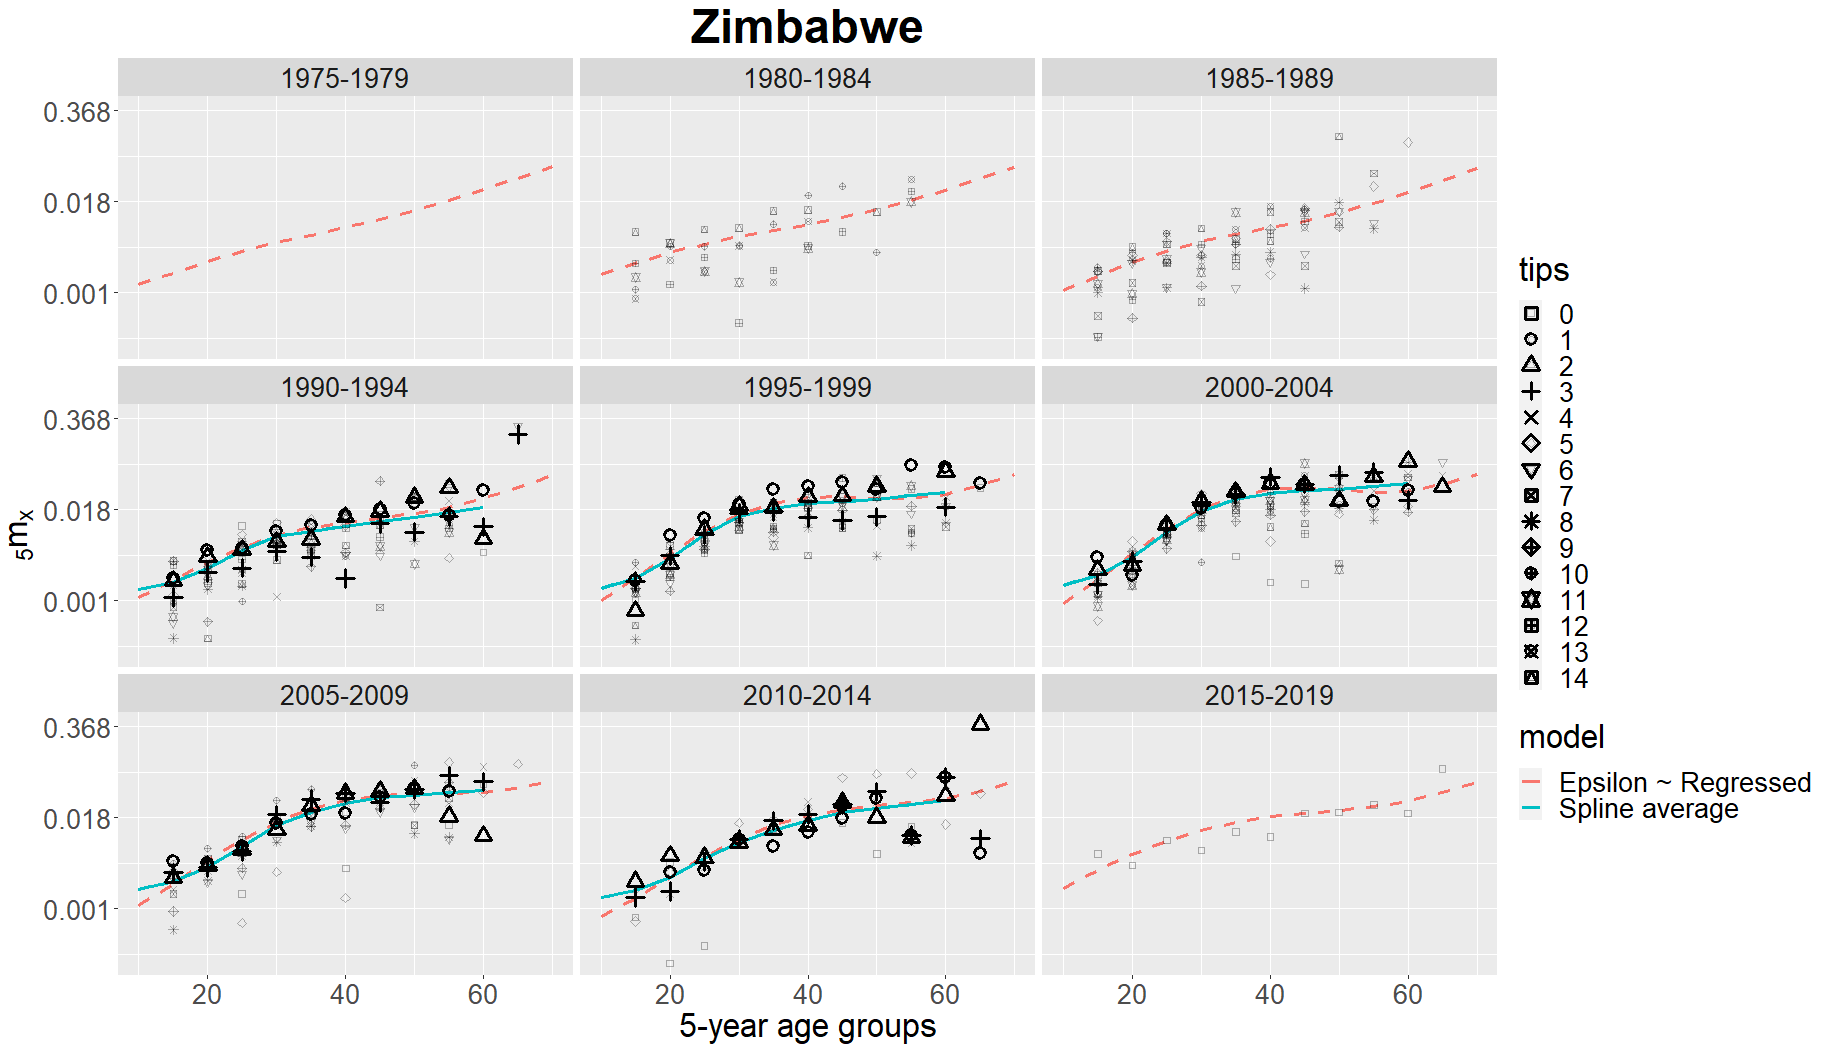
\includegraphics[width = \linewidth]{Burkina Faso/9/Zimbabwe male.png}
\caption*{Males}
\end{figure}
\begin{figure}[H]
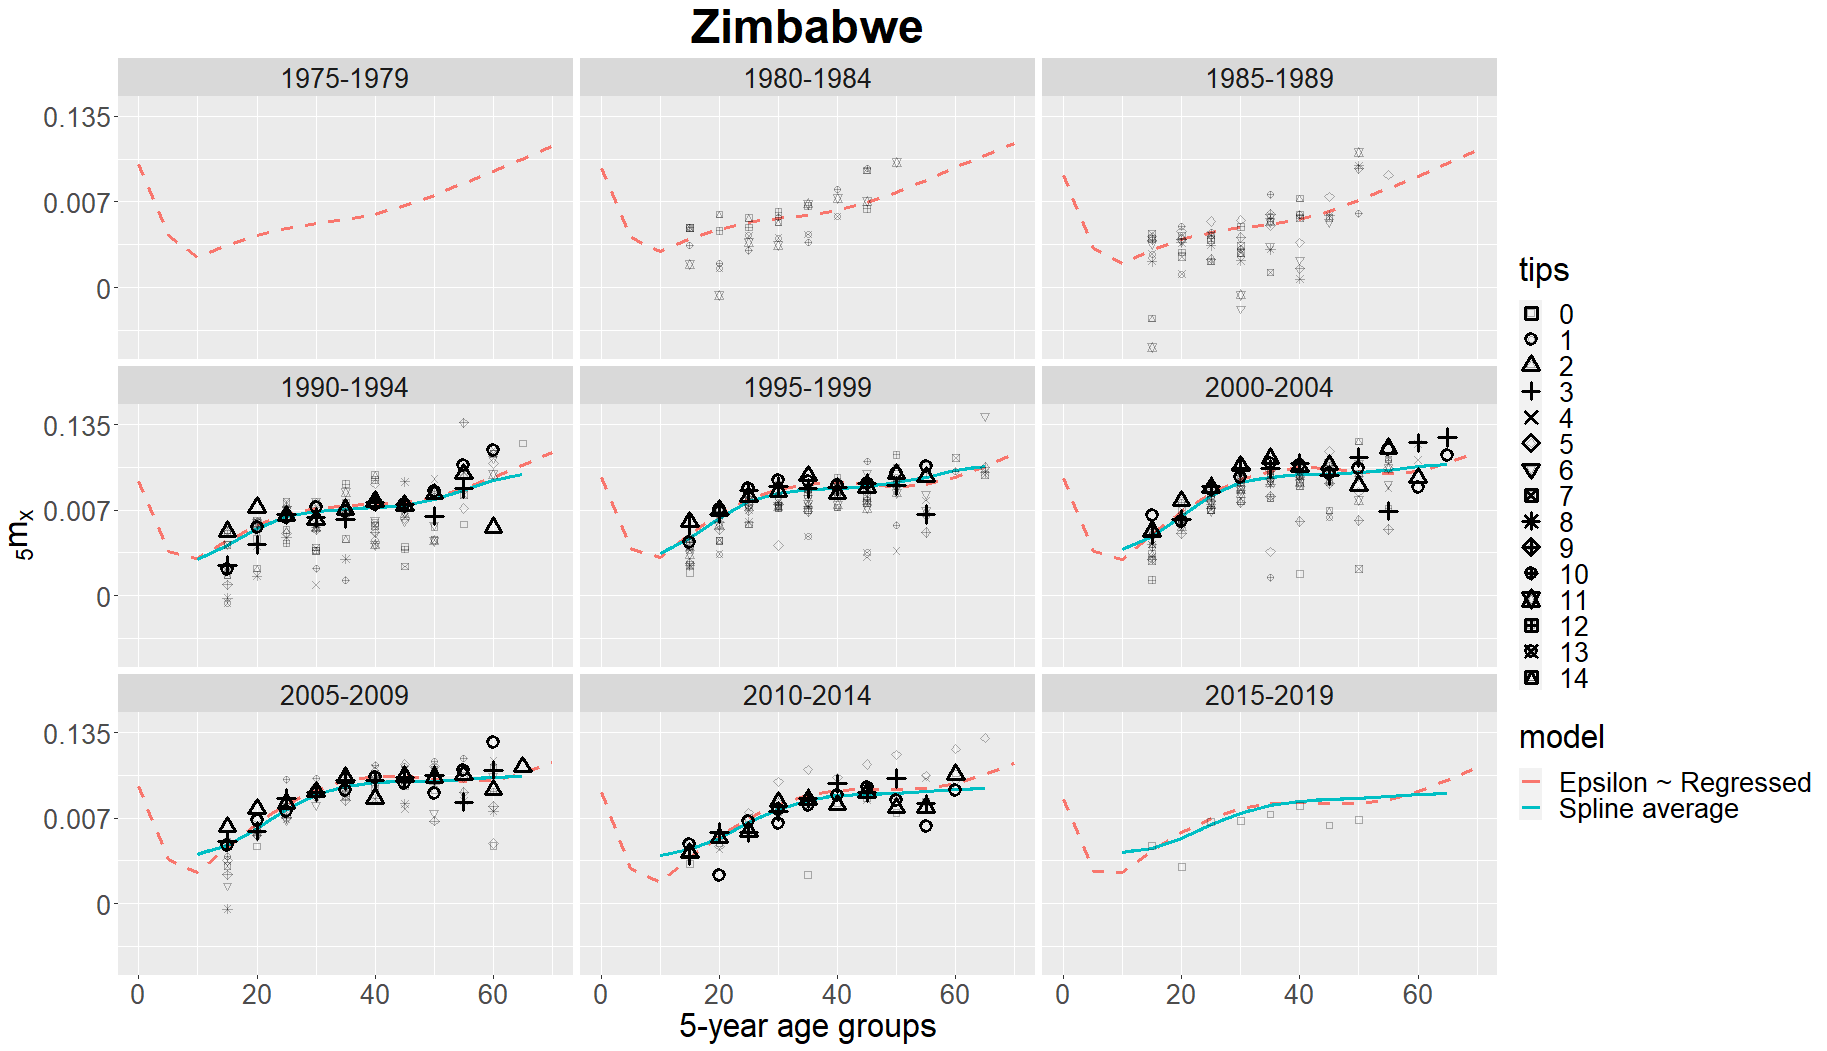
\includegraphics[width = \linewidth]{Burkina Faso/9/Zimbabwe female.png}
\caption*{Females}
\end{figure}
\begin{itemize}
\item Splines seem to over-smooth the hump
\end{itemize}

\end{document} 